\begin{multicols*}{2}

\section{Part 1}
All algorithms were implemented without transforming and storing the maze into a tree. Instead, for each coordinate visited, each of its four neighbors are treated as the current coordinate's children, and are visited and added to the frontier if not already visited. All algorithms terminate when the current coordinate being examined is the goal since looking any further into its neighbors would only yield longer paths and potentially repeated states.
\subsection*{1.1}
\subsubsection*{Breadth-first search}
Our breadth-first search algorithm uses a FIFO queue to keep track of which coordinates in the maze are in the frontier. We also keep a list of coordinates that have been visited, and a queue of paths that are the paths from the start to the corresponding coordinates for each of the neighbors of a coordinate. For each path in the frontier, our algorithm visits its four neighbor coordinates and checks whether each is within the maze boundaries, is not a wall or ghost, and has not been visited yet. If a neighbor coordinate satisfies these conditions, it is added to the frontier by appending to the (right) end of the queue, and the path to it is added to the path queue so that it can be referenced later to compute the path to its own neighbors. Once the four neighbors of a coordinate have been added to the frontier, if applicable, the algorithm moves on to examine the next coordinate in the frontier by popping the leftmost coordinate in the frontier.

To get the path for the current neighbor being examined, the leftmost path in the the queue of paths is popped. Since each of a coordinate's neighbors is appended to the frontier at the same time as when the path to said neighbor is appended to the queue of paths, the path popped from the path queue always corresponds to the coordinate being popped from the frontier.

\paragraph{Results}
smallTurn.txt\\
- Path cost: 53\\
- Number of nodes expanded: 162\\
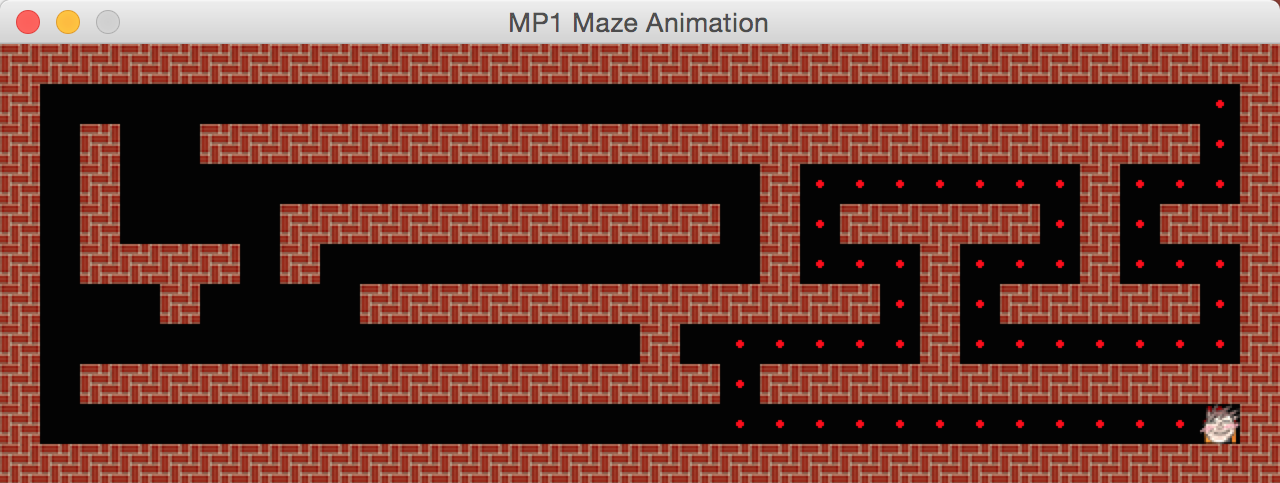
\includegraphics[width=0.3\textwidth]{graphics/smallTurn_bfs.png}

\paragraph{Results}
mediumMaze.txt\\
- Path cost: 43\\
- Number of nodes expanded: 227\\
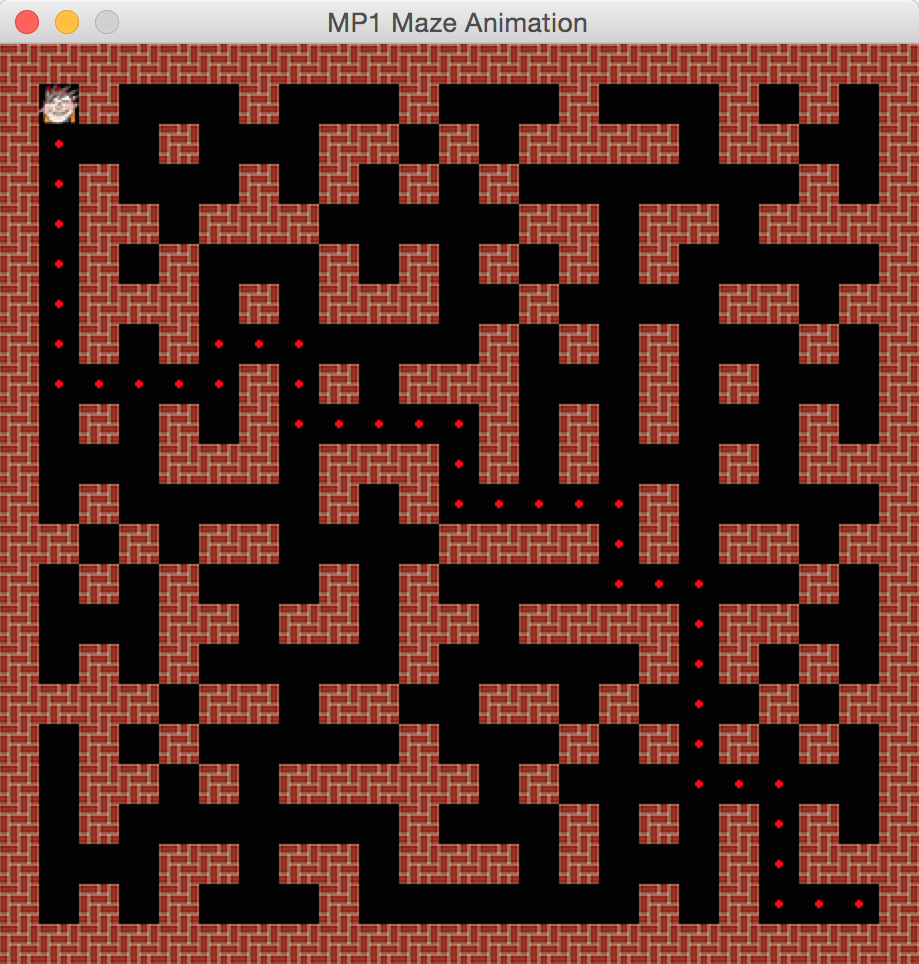
\includegraphics[width=0.3\textwidth]{graphics/mediumMaze_bfs.png}

\columnbreak
\paragraph{Results}
bigMaze.txt\\
- Path cost: 63\\
- Number of nodes expanded: 730\\
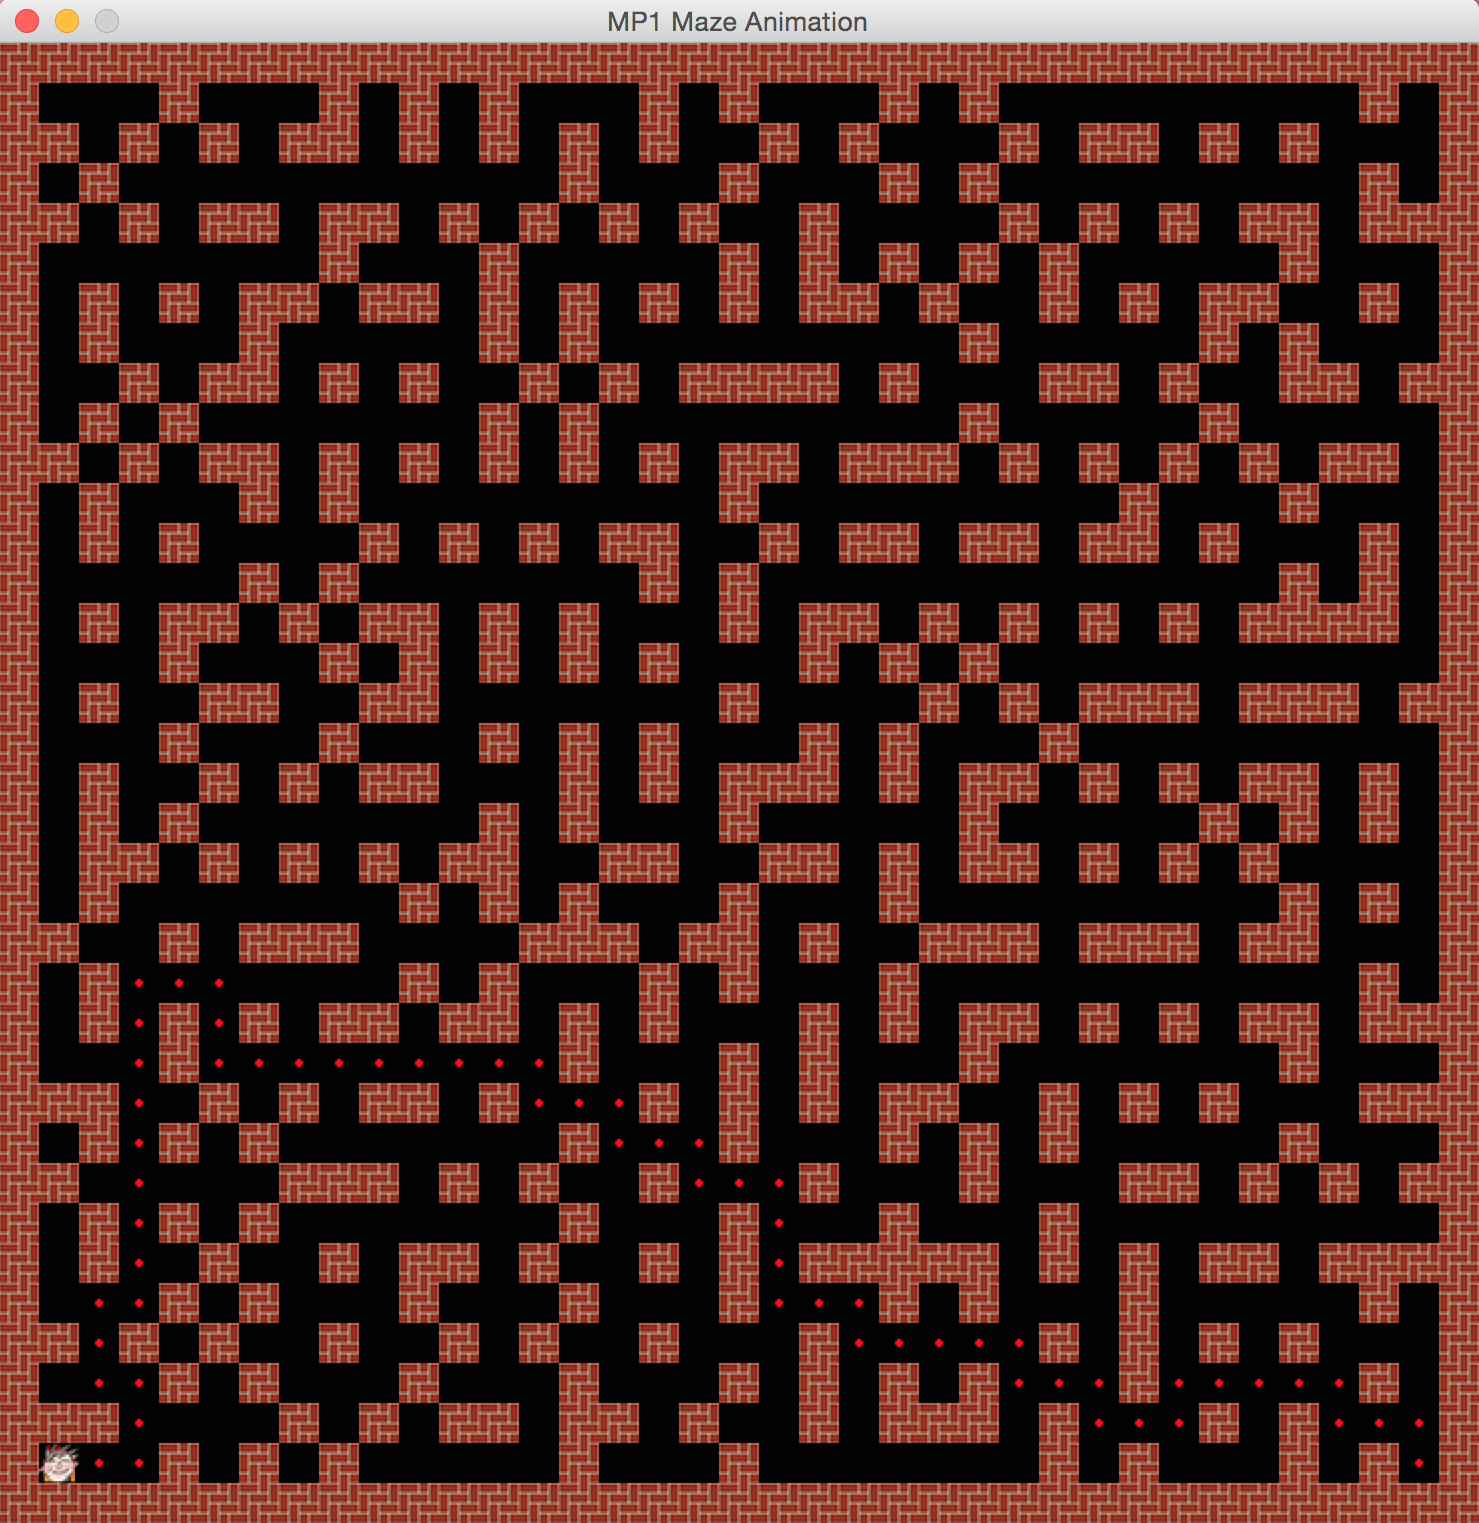
\includegraphics[width=0.3\textwidth]{graphics/bigMaze_bfs.png}

\paragraph{Results}
openMaze.txt\\
- Path cost: 55\\
- Number of nodes expanded: 302\\
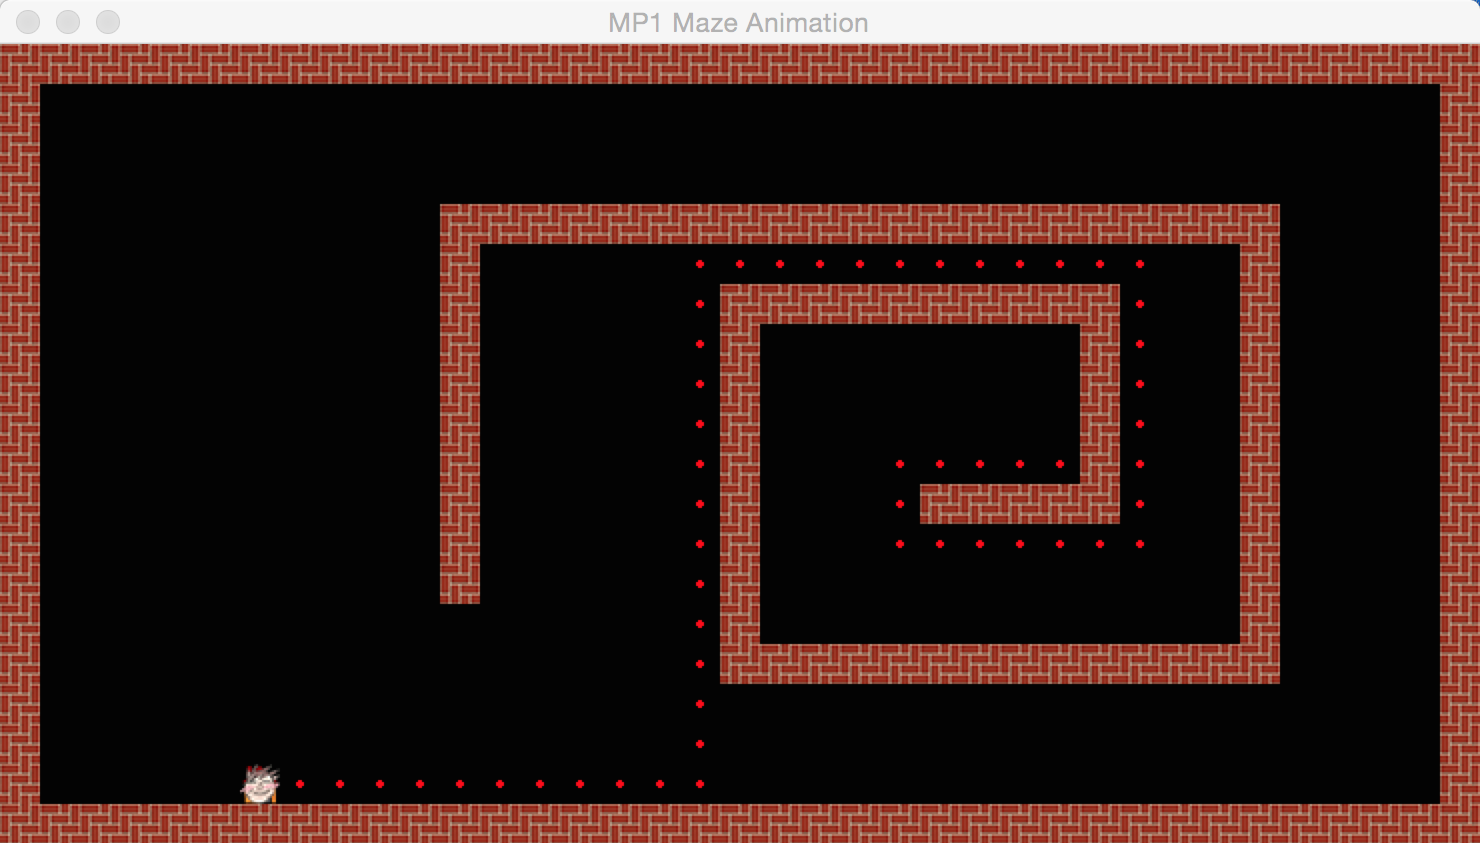
\includegraphics[width=0.3\textwidth]{graphics/openMaze_bfs.png}

\subsubsection*{Depth-first search}
Our depth-first search algorithm is similar to our BFS algorithm but uses a LIFO stack to keep track of the frontier coordinates and the corresponding paths to them. This way, the algorithm visits a coordinate's neighbors before other coordinates at the same level. By our array representation of the maze, two coordinates are considered to be on the same level if they were both neighbors of the same coordinate and were both visited when that coordinate was popped from the frontier.

There was no other difference between our BFS and DFS code since the use of a stack instead of a queue to store the coordinates in the frontier marks the main difference between DFS and BFS.

\paragraph{Results}
smallTurn.txt\\
- Path cost: 67\\
- Number of nodes expanded: 111\\
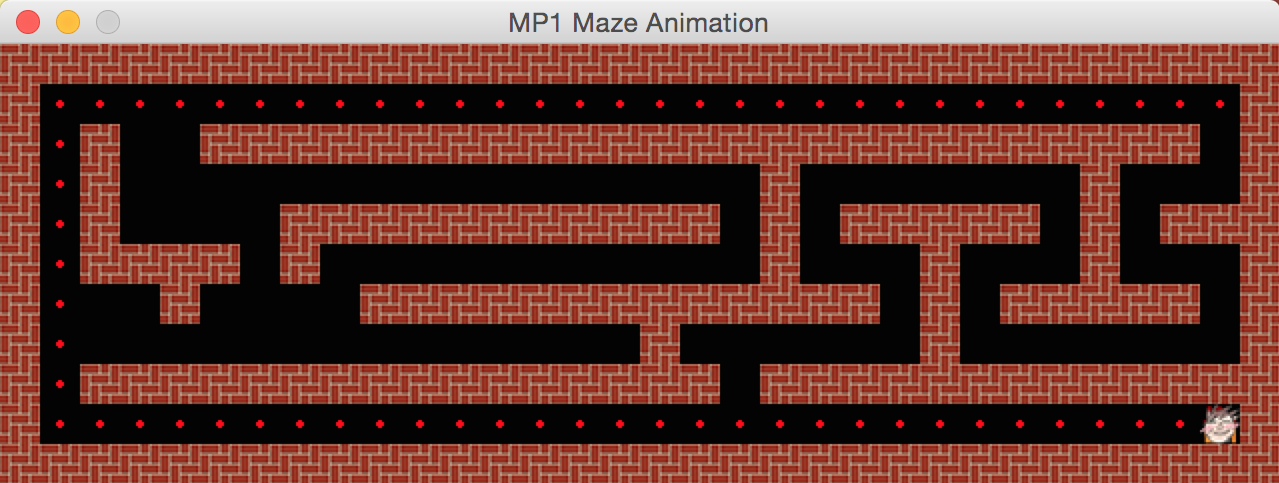
\includegraphics[width=0.3\textwidth]{graphics/smallTurn_dfs.png}

\paragraph{Results}
mediumMaze.txt\\
- Path cost: 65\\
- Number of nodes expanded: 99\\
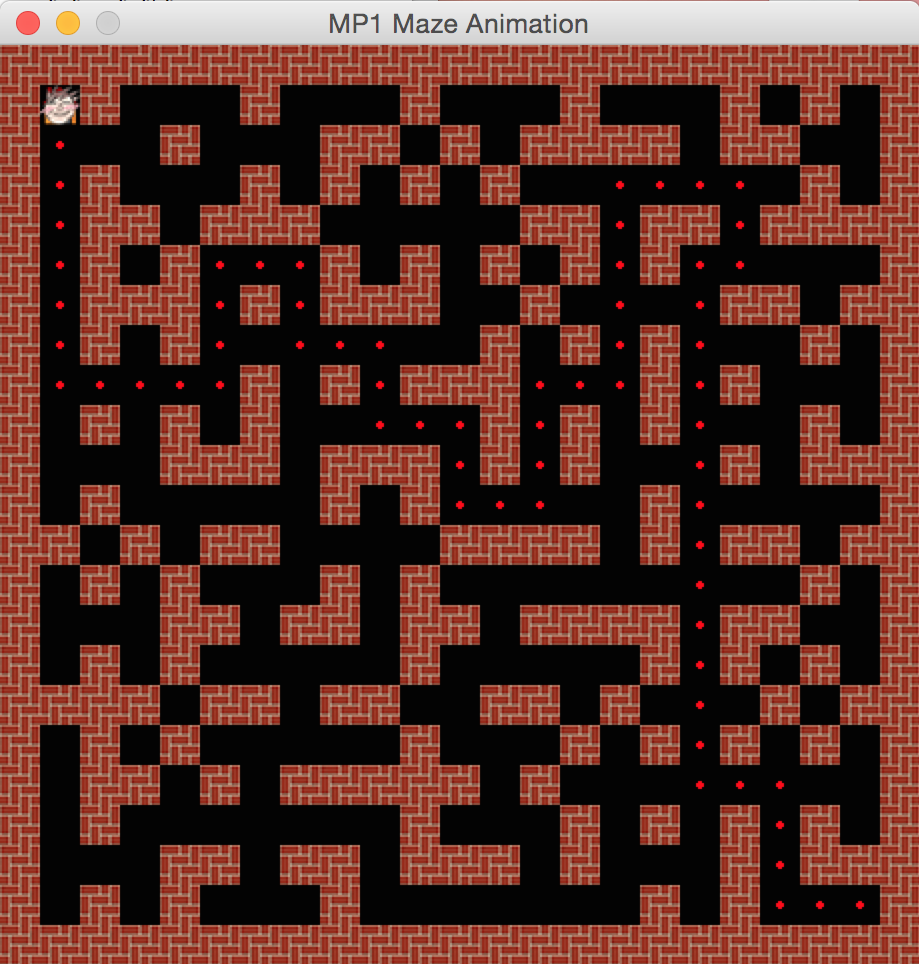
\includegraphics[width=0.3\textwidth]{graphics/mediumMaze_dfs.png}

\paragraph{Results}
bigMaze.txt\\
- Path cost: 155\\
- Number of nodes expanded: 352\\
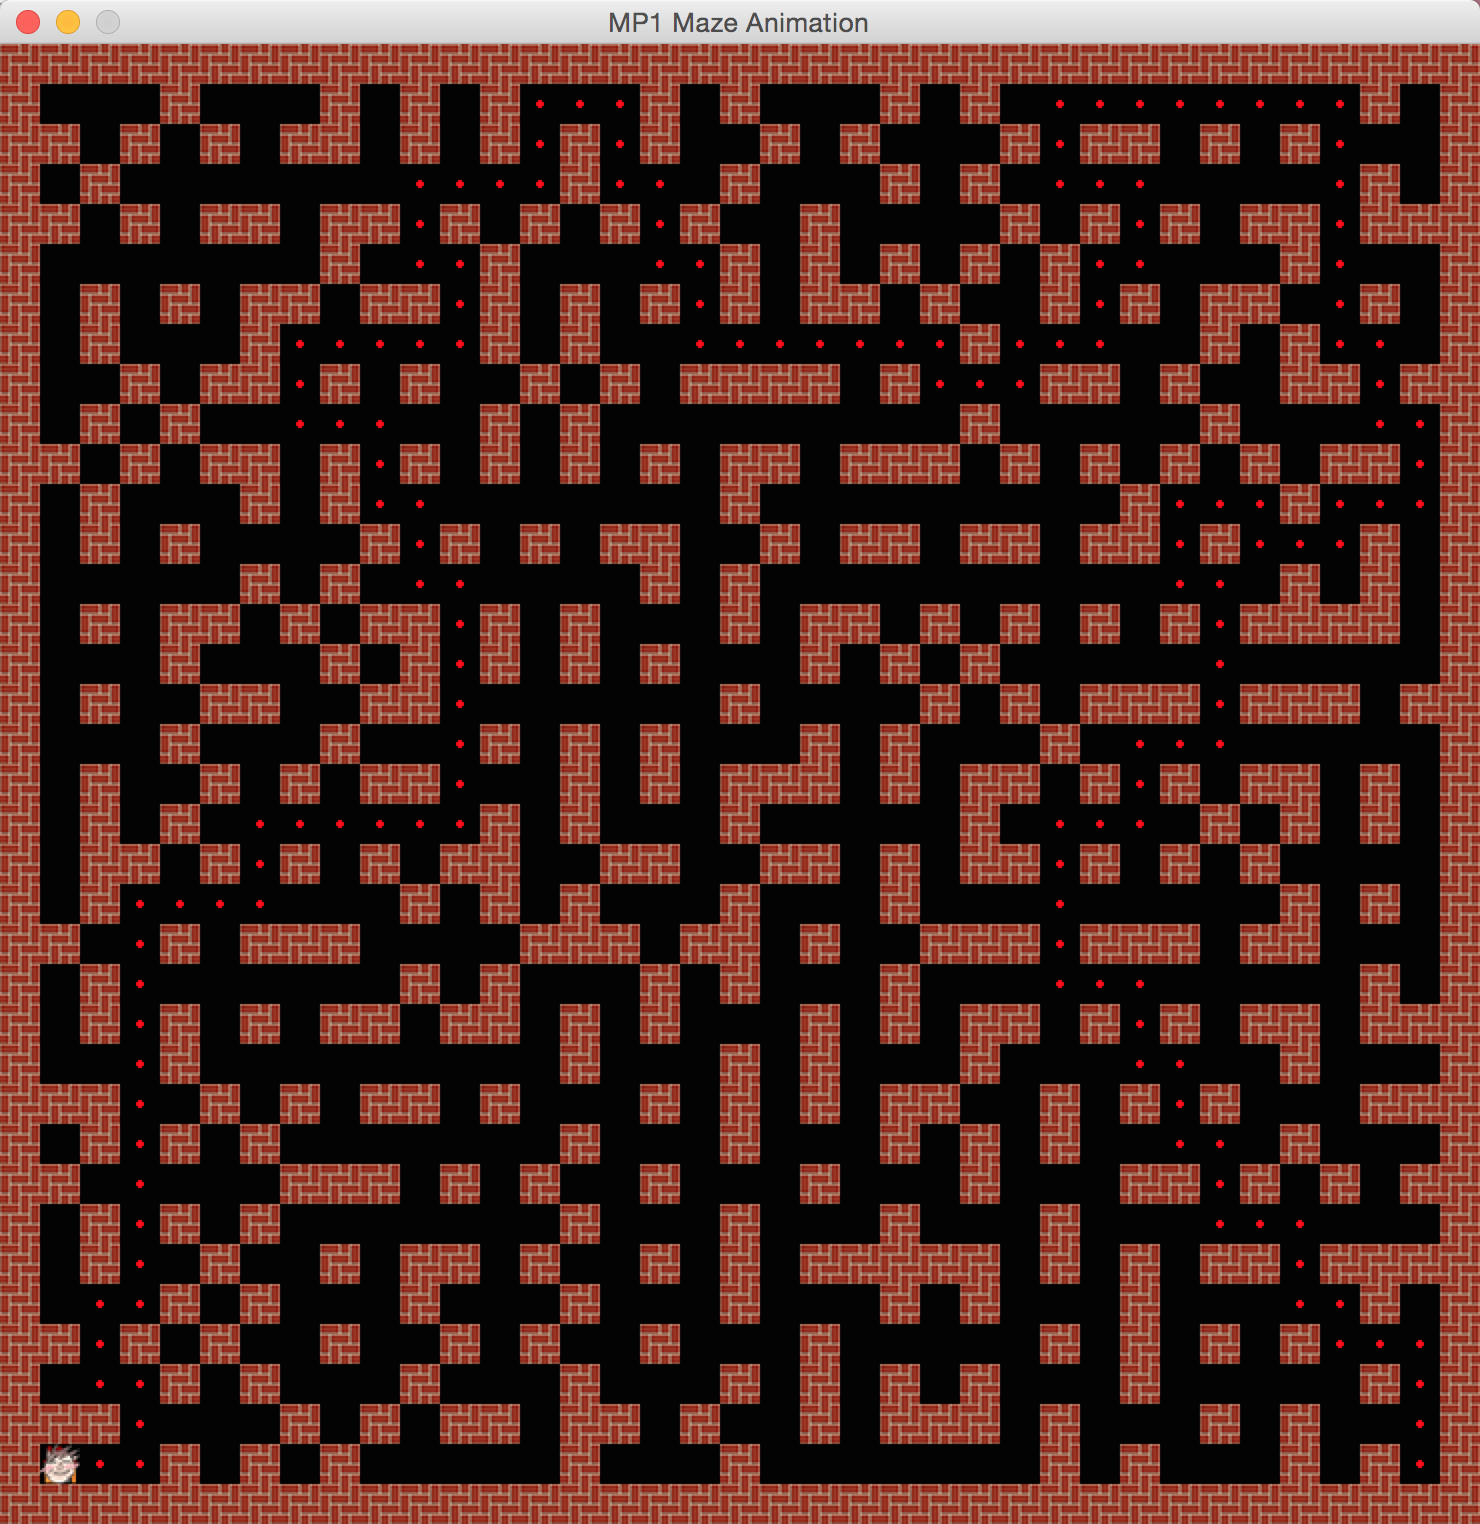
\includegraphics[width=0.3\textwidth]{graphics/bigMaze_dfs.png}

\columnbreak
\paragraph{Results}
openMaze.txt\\
- Path cost: 147\\
- Number of nodes expanded: 278\\
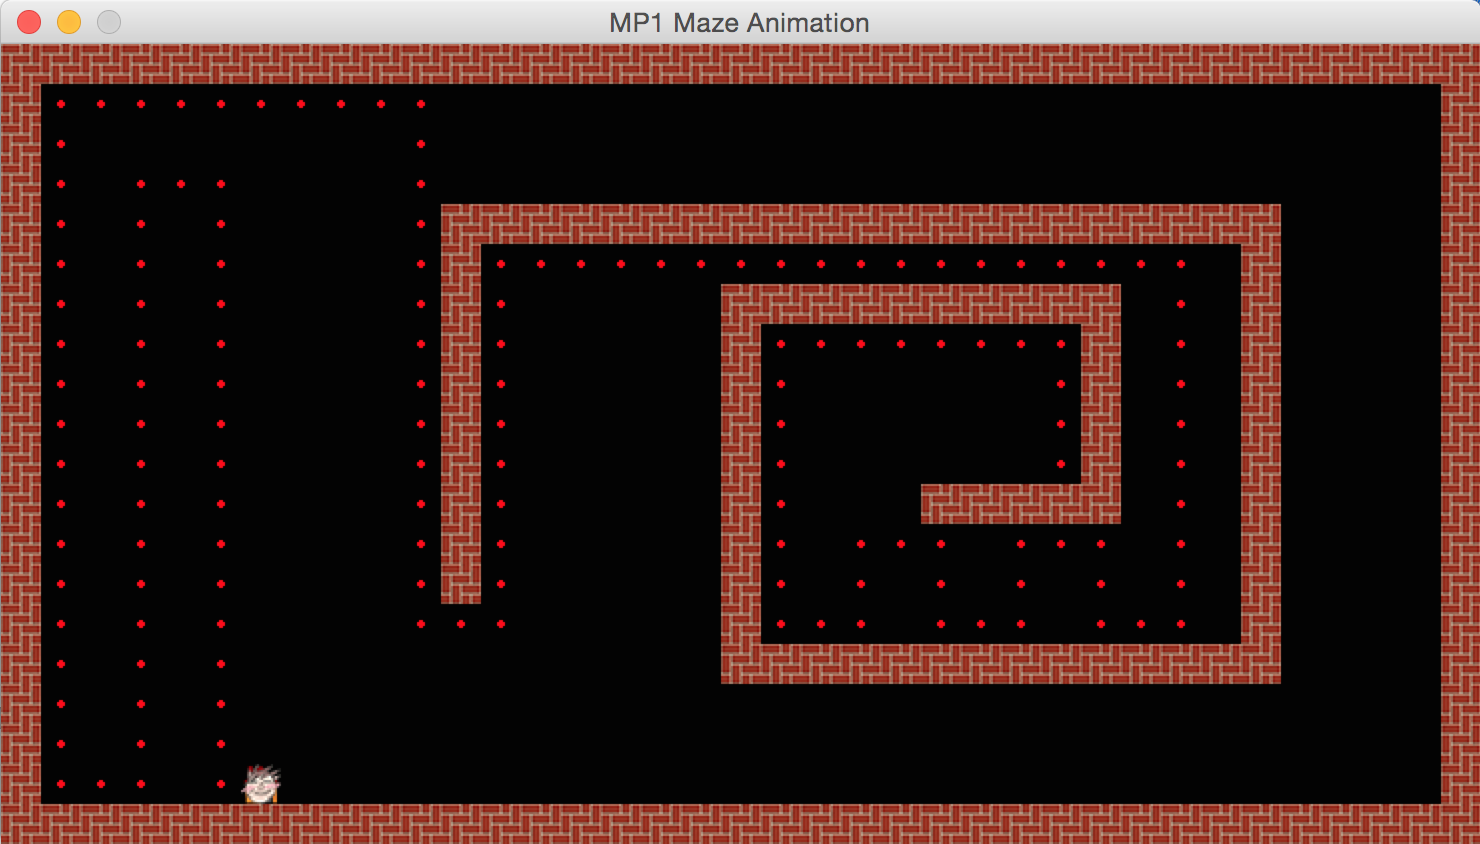
\includegraphics[width=0.3\textwidth]{graphics/openMaze_dfs.png}

\subsubsection*{Greedy best-first search}
Our greedy best-first search uses a min-heap to track the coordinates in the frontier, where objects are ordered in the heap by their Manhattan distance from the goal. However, since the heap needs to store the Manhattan distance in addition to the coordinate, instead of just storing the coordinate in the frontier like in BFS and DFS, the algorithm stores tuples of the form (Manhattan distance from current coordinate to the goal, path from start to current coordinate, current coordinate).

The greedy algorithm then pops from the frontier the coordinate's tuple that has the lowest Manhattan distance to the goal of all coordinates in the frontier and examines its neighbors, adding them to the frontier as tuples, if applicable. The algorithm then continues examining the frontier as described, expanding the coordinate with the lowest Manhattan distance first.

\paragraph{Results}
smallTurn.txt\\
- Path cost: 53\\
- Number of nodes expanded: 64\\
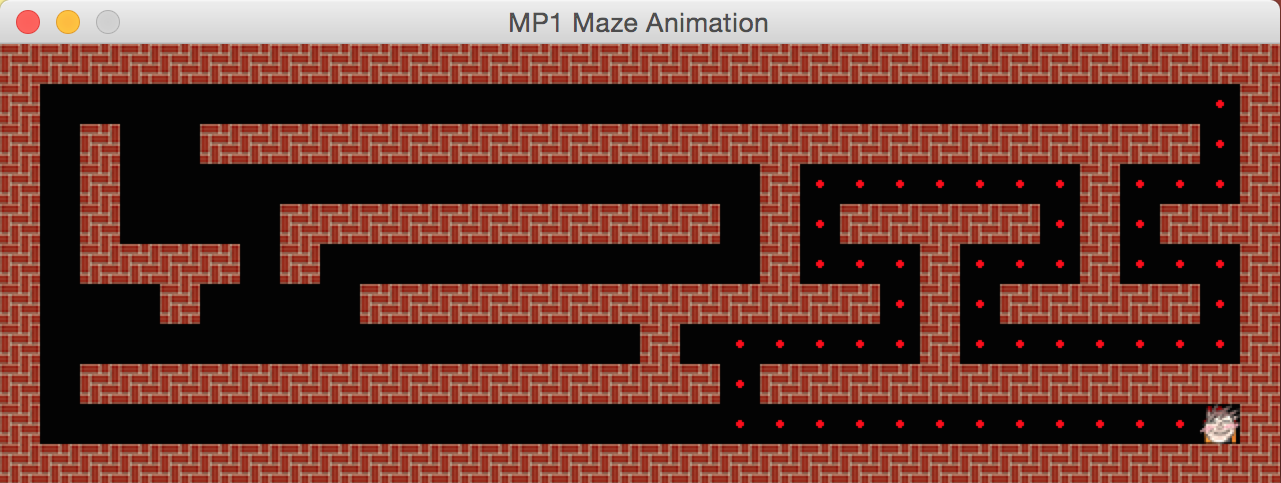
\includegraphics[width=0.3\textwidth]{graphics/smallTurn_greedy.png}

\paragraph{Results}
mediumMaze.txt\\
- Path cost: 57\\
- Number of nodes expanded: 100\\
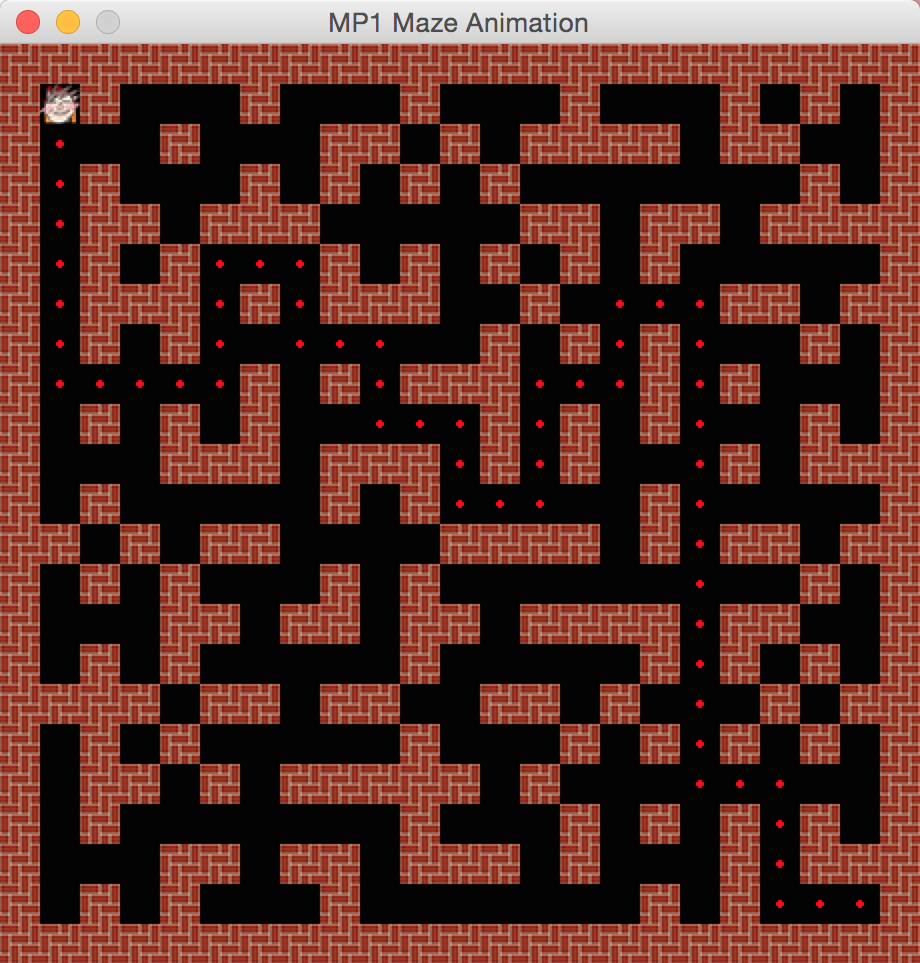
\includegraphics[width=0.3\textwidth]{graphics/mediumMaze_greedy.png}

\paragraph{Results}
bigMaze.txt\\
- Path cost: 71\\
- Number of nodes expanded: 151\\
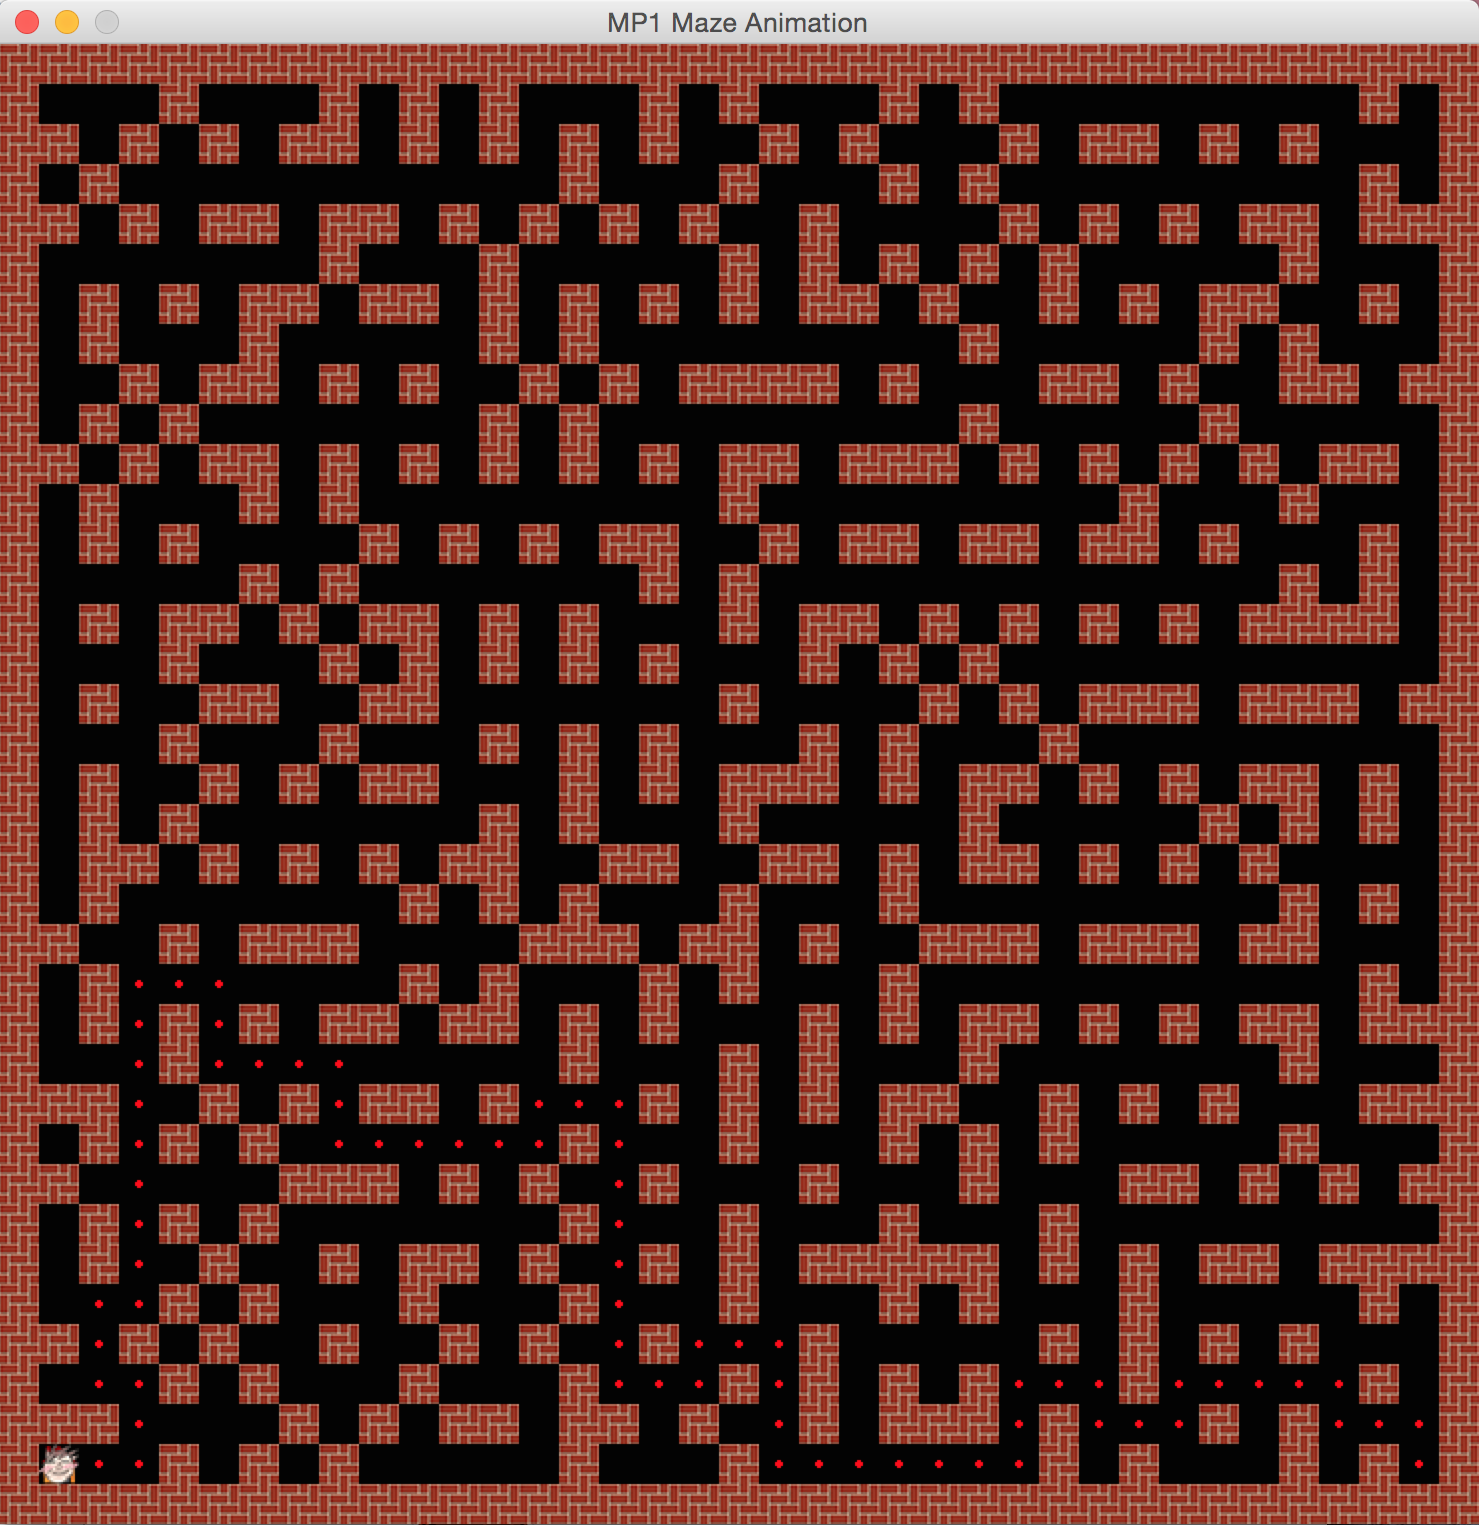
\includegraphics[width=0.3\textwidth]{graphics/bigMaze_greedy.png}

\paragraph{Results}
openMaze.txt\\
- Path cost: 61\\
- Number of nodes expanded: 156\\
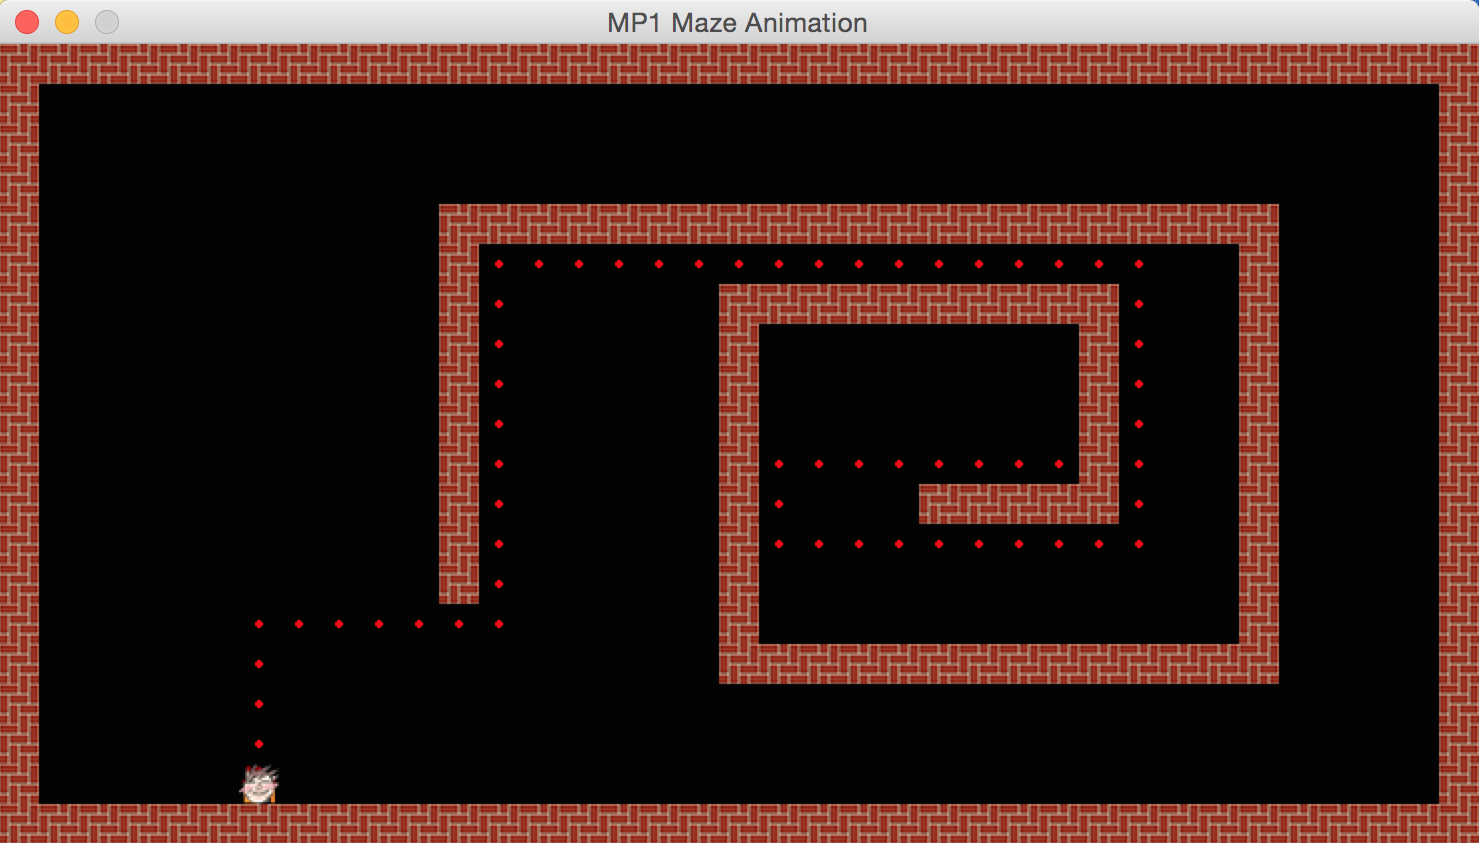
\includegraphics[width=0.3\textwidth]{graphics/openMaze_greedy.png}

\subsubsection*{A*}
Our A* algorithm is similar to our greedy best-first search in that it also uses a min-heap of tuples storing coordinate data. However, this heap is ordered by the sum of the path cost to the coordinate plus the Manhattan distance from there to the goal since the A* algorithm takes that as the heuristic instead of just Manhattan distance. A* uses this heuristic so that it avoids expanding coordinates with larger path costs to them from the maze start.

Therefore, this algorithm stores in the heap tuples of the form (path cost from start to this coordinate plus Manhattan distance from here to goal, path cost from start to this coordinate, path from start to this coordinate, this coordinate). A* pops from the frontier the coordinate's tuple with the lowest path cost plus Manhattan distance and examines its neighbors, adding them to the frontier as tuples if they are within the maze boundaries and have not been visited. The algorithm then continues examining the frontier as described, expanding the coordinate with the lowest sum of current path cost and Manhattan distance heuristic.

\paragraph{Results}
smallTurn.txt\\
- Path cost: 53\\
- Number of nodes expanded: 78\\
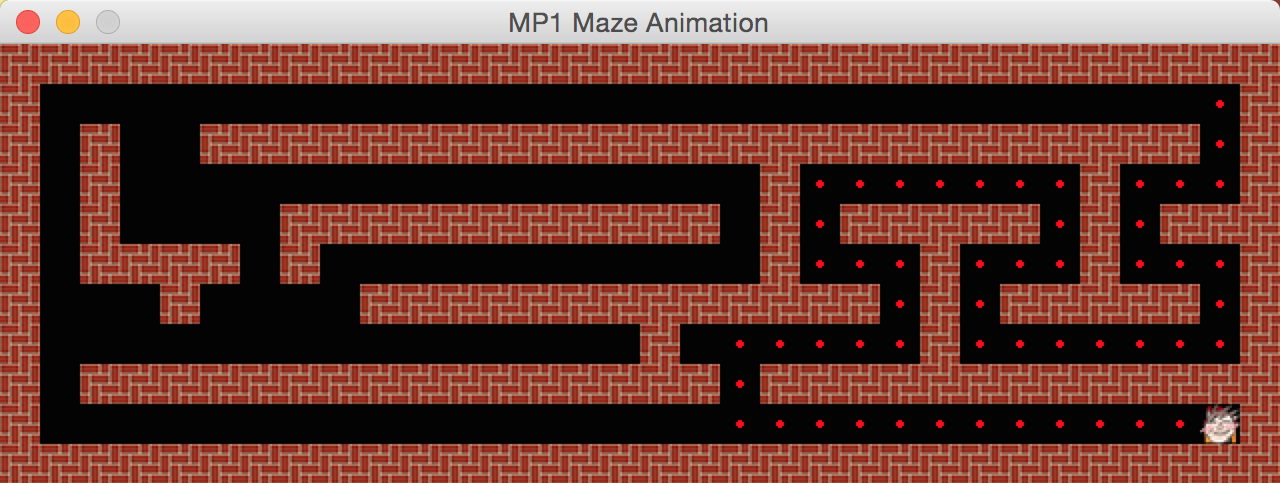
\includegraphics[width=0.3\textwidth]{graphics/smallTurn_astar.png}

\paragraph{Results}
mediumMaze.txt\\
- Path cost: 43\\
- Number of nodes expanded: 124\\
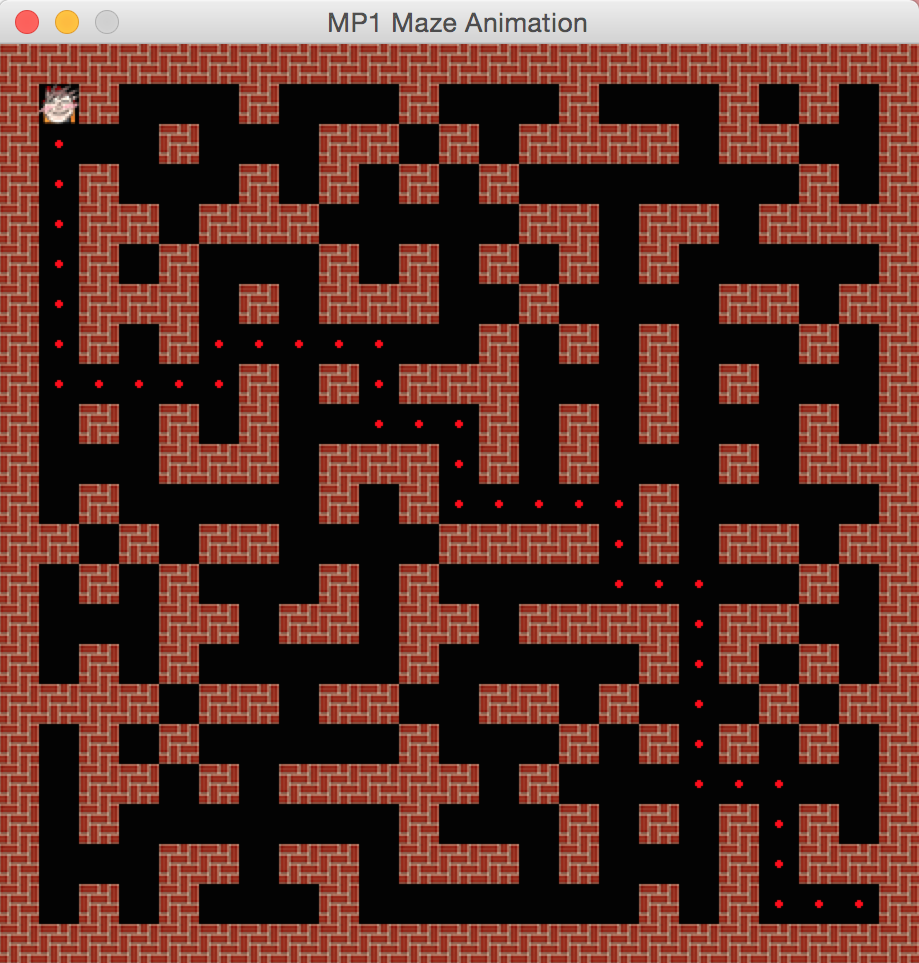
\includegraphics[width=0.3\textwidth]{graphics/mediumMaze_astar.png}

\paragraph{Results}
bigMaze.txt\\
- Path cost: 63\\
- Number of nodes expanded: 308\\
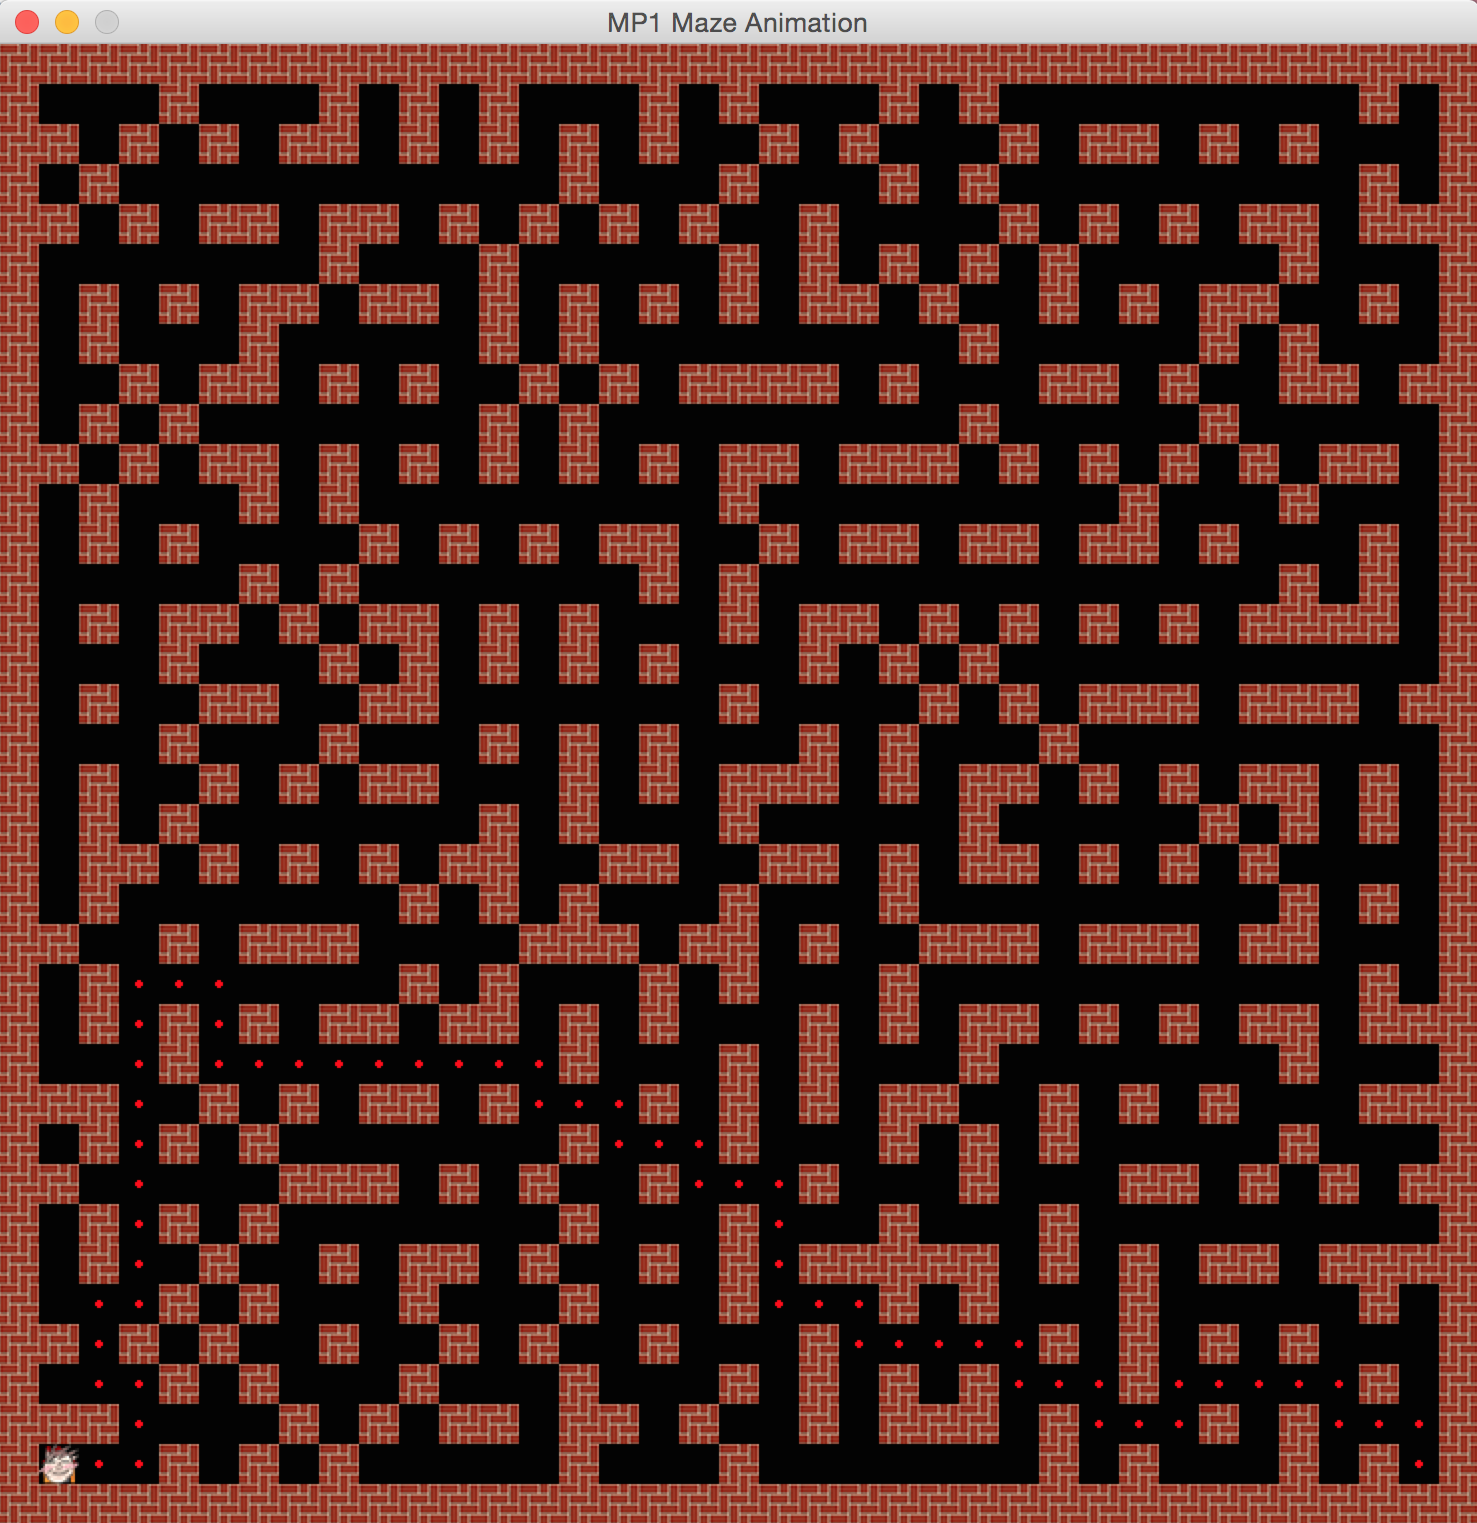
\includegraphics[width=0.3\textwidth]{graphics/bigMaze_astar.png}

\paragraph{Results}
openMaze.txt\\
- Path cost: 55\\
- Number of nodes expanded: 228\\
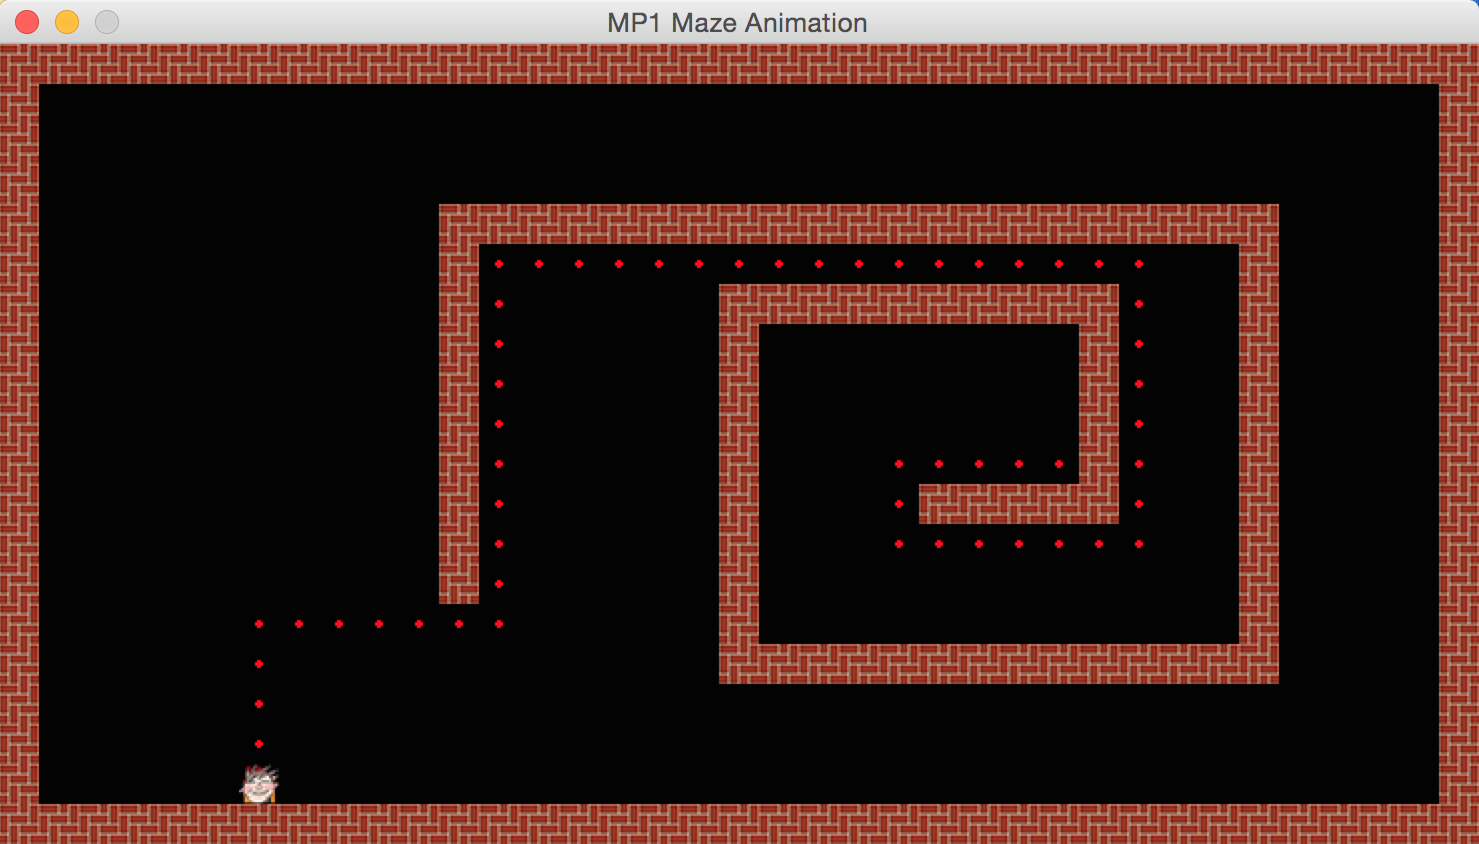
\includegraphics[width=0.3\textwidth]{graphics/openMaze_astar.png}

\subsection*{1.2}
Our alternative heuristic returns the Manhattan distance from the current coordinate to the goal multiplied by the move cost, plus the turn cost multiplied by the number of times Pacman must turn from his current direction and position at the neighbor coordinate being examined to reach the goal via a Manhattan route. At most, Pacman must turn twice: once to face the correct first direction to move towards the goal in that dimension, and once to orient himself along the second dimension. If Pacman already has the correct coordinate AND direction in one dimension, he does not need to make any turns since he can go straight in that one direction to reach the goal. If Pacman already has just the correct coordinate in one dimension, he needs to make a single turn and then go straight in that one dimension.

Once the number of turns Pacman needs to make is computed, the Manhattan portion of the heuristic is computed and the value for the heuristic returned.

This heuristic is admissible since it ignores walls, so the cost of movement is always less than or equal to the actual cost of movement. Since the heuristic ignores walls, the cost of turning is also always less than or equal to the actual cost of turns required to move from the current coordinate to the goal. With walls, Pacman may need to make more turns to get around the walls, but using the Manhattan route from the current coordinate to the goal requires only the (minimum) number of turns needed to orient Pacman in the direction of the goal, which would have been required with walls as well. Therefore, Pacman must make those turns in the actual solution path as well, in addition to any other turns required to maneuver around walls, so Pacman must take at least that number of turns computed for our heuristic.

This heuristic is more informed than Manhattan distance since it takes into account the cost of turning. Therefore, the heuristic will favor neighbors where Pacman is facing in the general direction of the goal when he moves there. This makes sense intuitively since having Pacman move to a neighbor where he is facing away from the goal would suggest that Pacman is moving away from the goal or maneuvering around many obstacles to get back to the goal.

\paragraph{Results}
smallTurns.txt, move cost = 2, turn cost = 1, Manhattan distance\\
- Path cost: 120\\
- Number of nodes expanded: 162\\
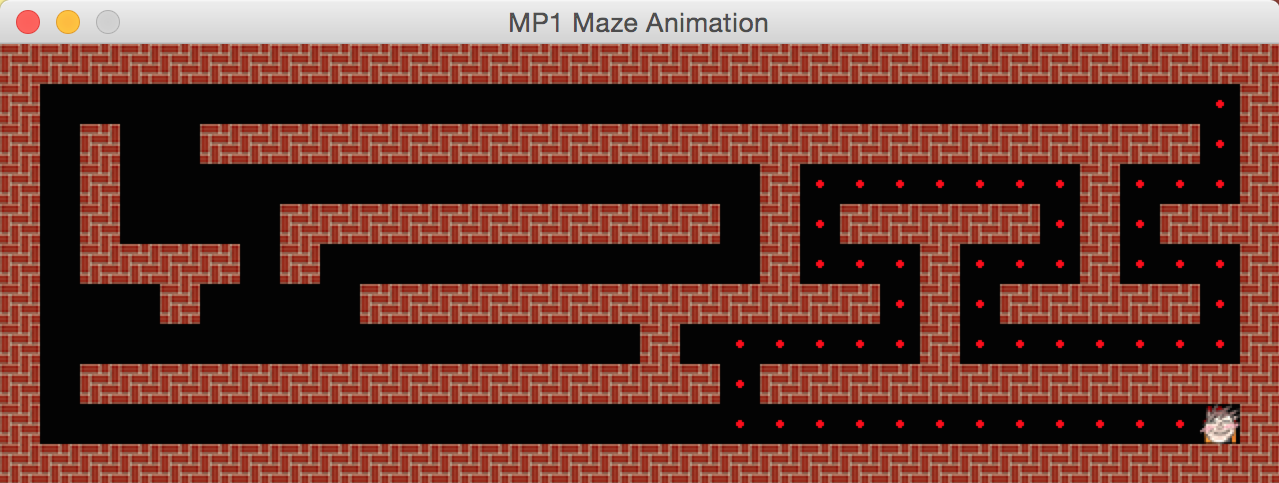
\includegraphics[width=0.3\textwidth]{graphics/smallTurn_turns21.png}

\paragraph{Results}
bigMaze.txt, move cost = 2, turn cost = 1, Manhattan distance\\
- Path cost: 152\\
- Number of nodes expanded: 570\\
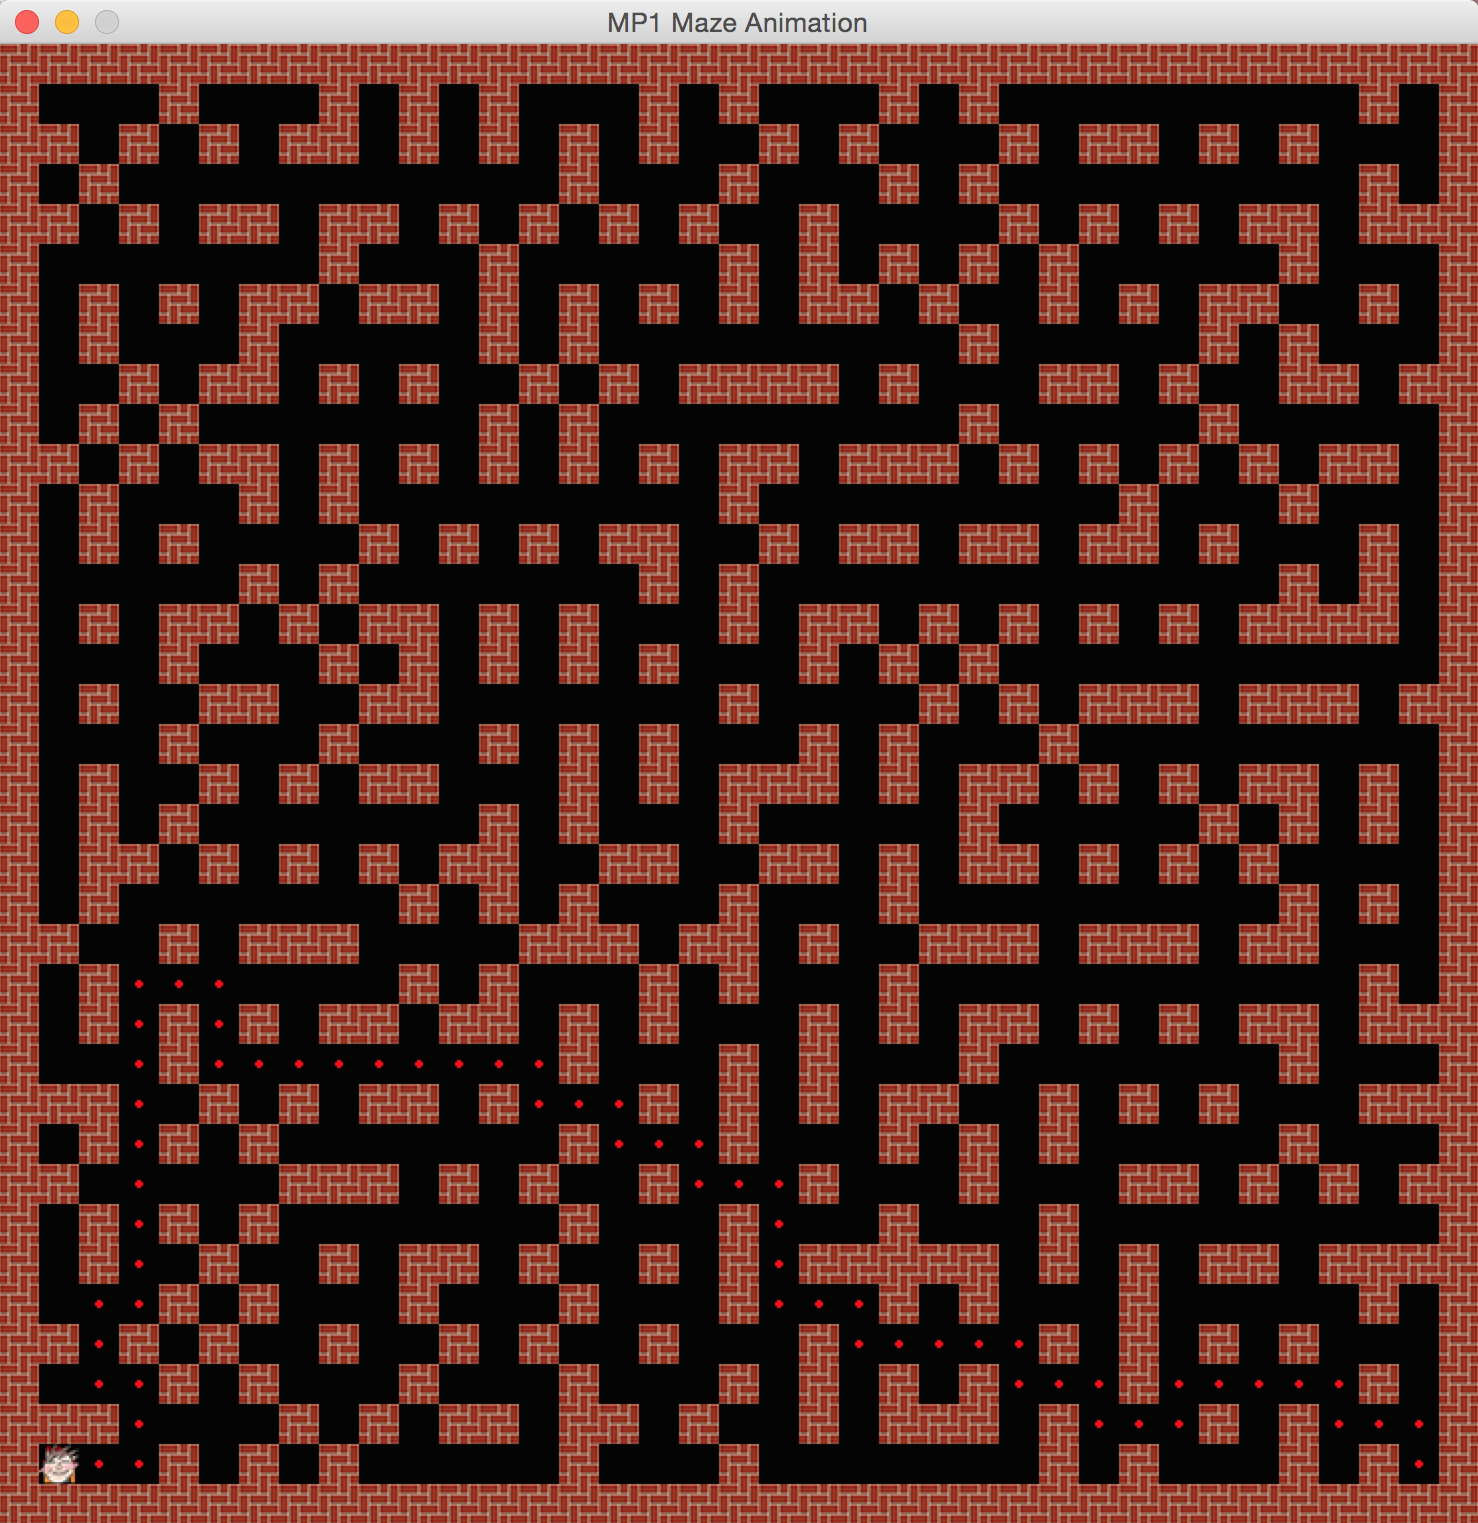
\includegraphics[width=0.3\textwidth]{graphics/bigMaze_turns21.png}

\paragraph{Results}
smallTurns.txt, move cost = 1, turn cost = 2, Manhattan distance\\
- Path cost: 74\\
- Number of nodes expanded: 146\\
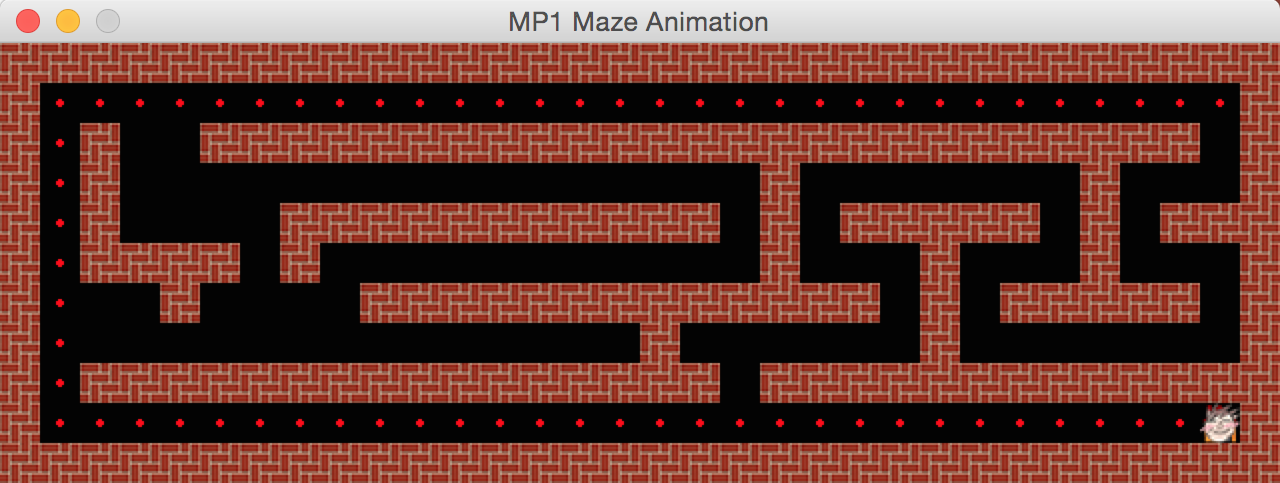
\includegraphics[width=0.3\textwidth]{graphics/smallTurn_turns12.png}

\paragraph{Results}
bigMaze.txt, move cost = 1, turn cost = 2, Manhattan distance\\
- Path cost: 118\\
- Number of nodes expanded: 537\\
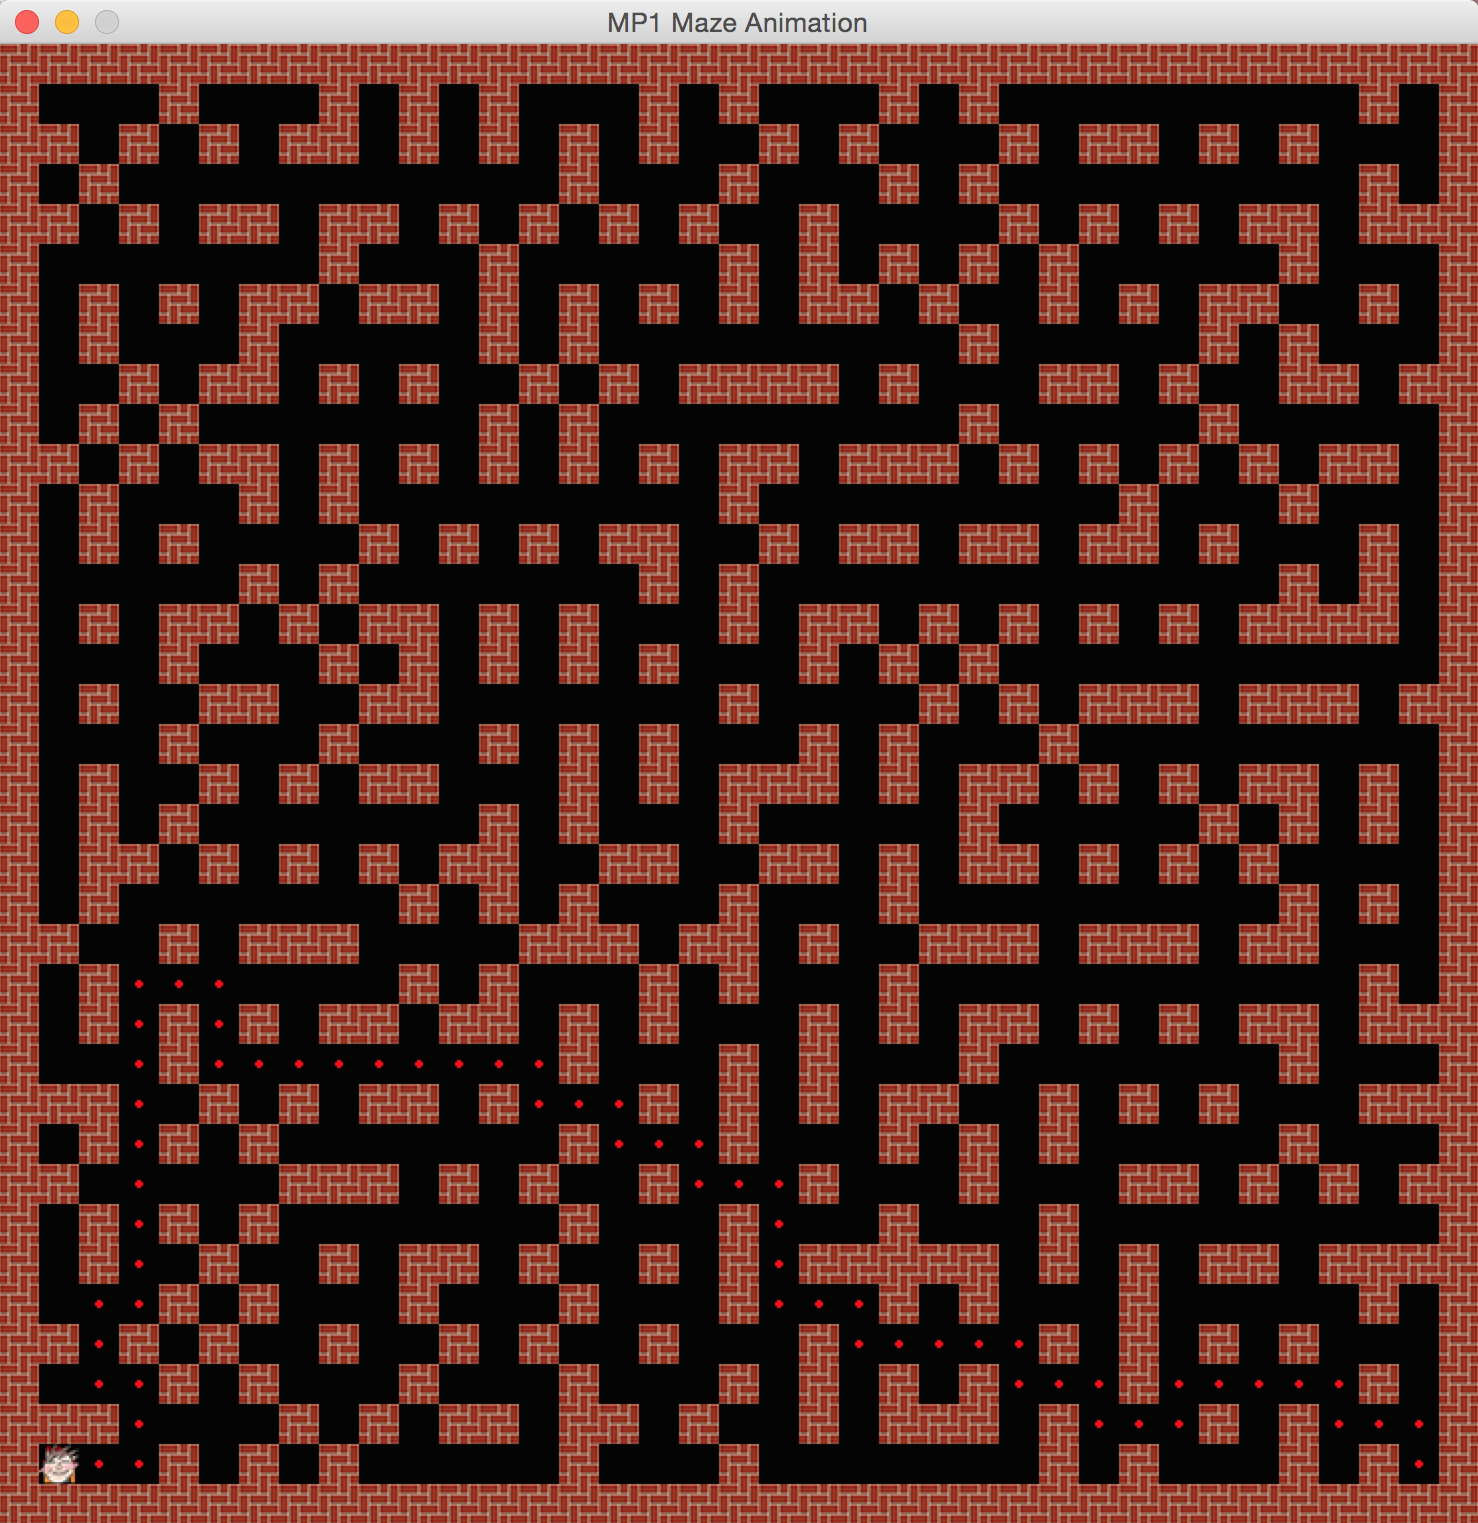
\includegraphics[width=0.3\textwidth]{graphics/bigMaze_turns12.png}

\paragraph{Results}
smallTurns.txt, move cost = 2, turn cost = 1, alternate heuristic\\
- Path cost: 120\\
- Number of nodes expanded: 81\\
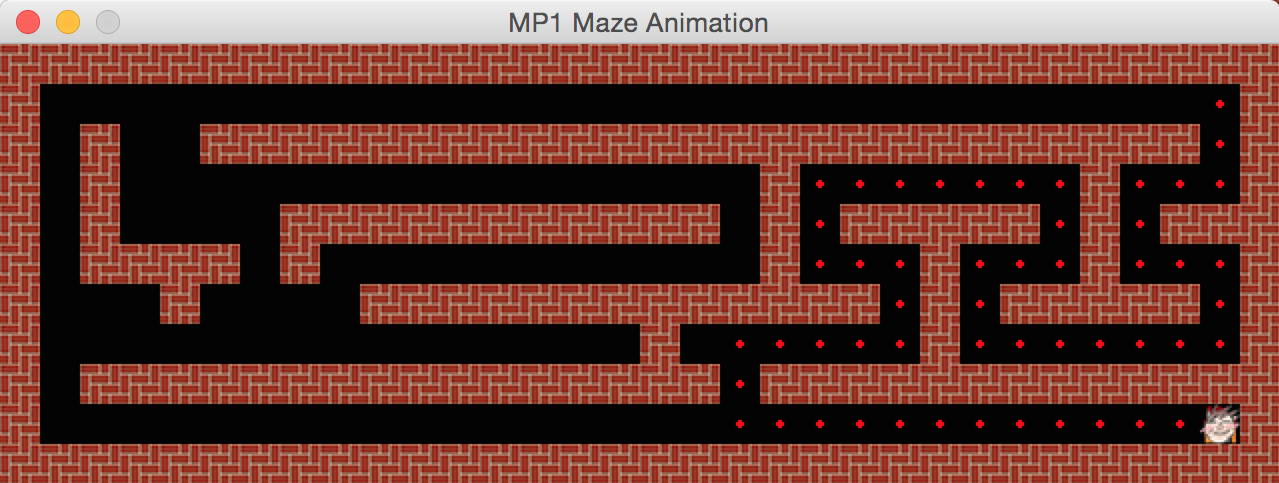
\includegraphics[width=0.3\textwidth]{graphics/smallTurn_alt21.png}

\paragraph{Results}
bigMaze.txt, move cost = 2, turn cost = 1, alternate heuristic\\
- Path cost: 152\\
- Number of nodes expanded: 347\\
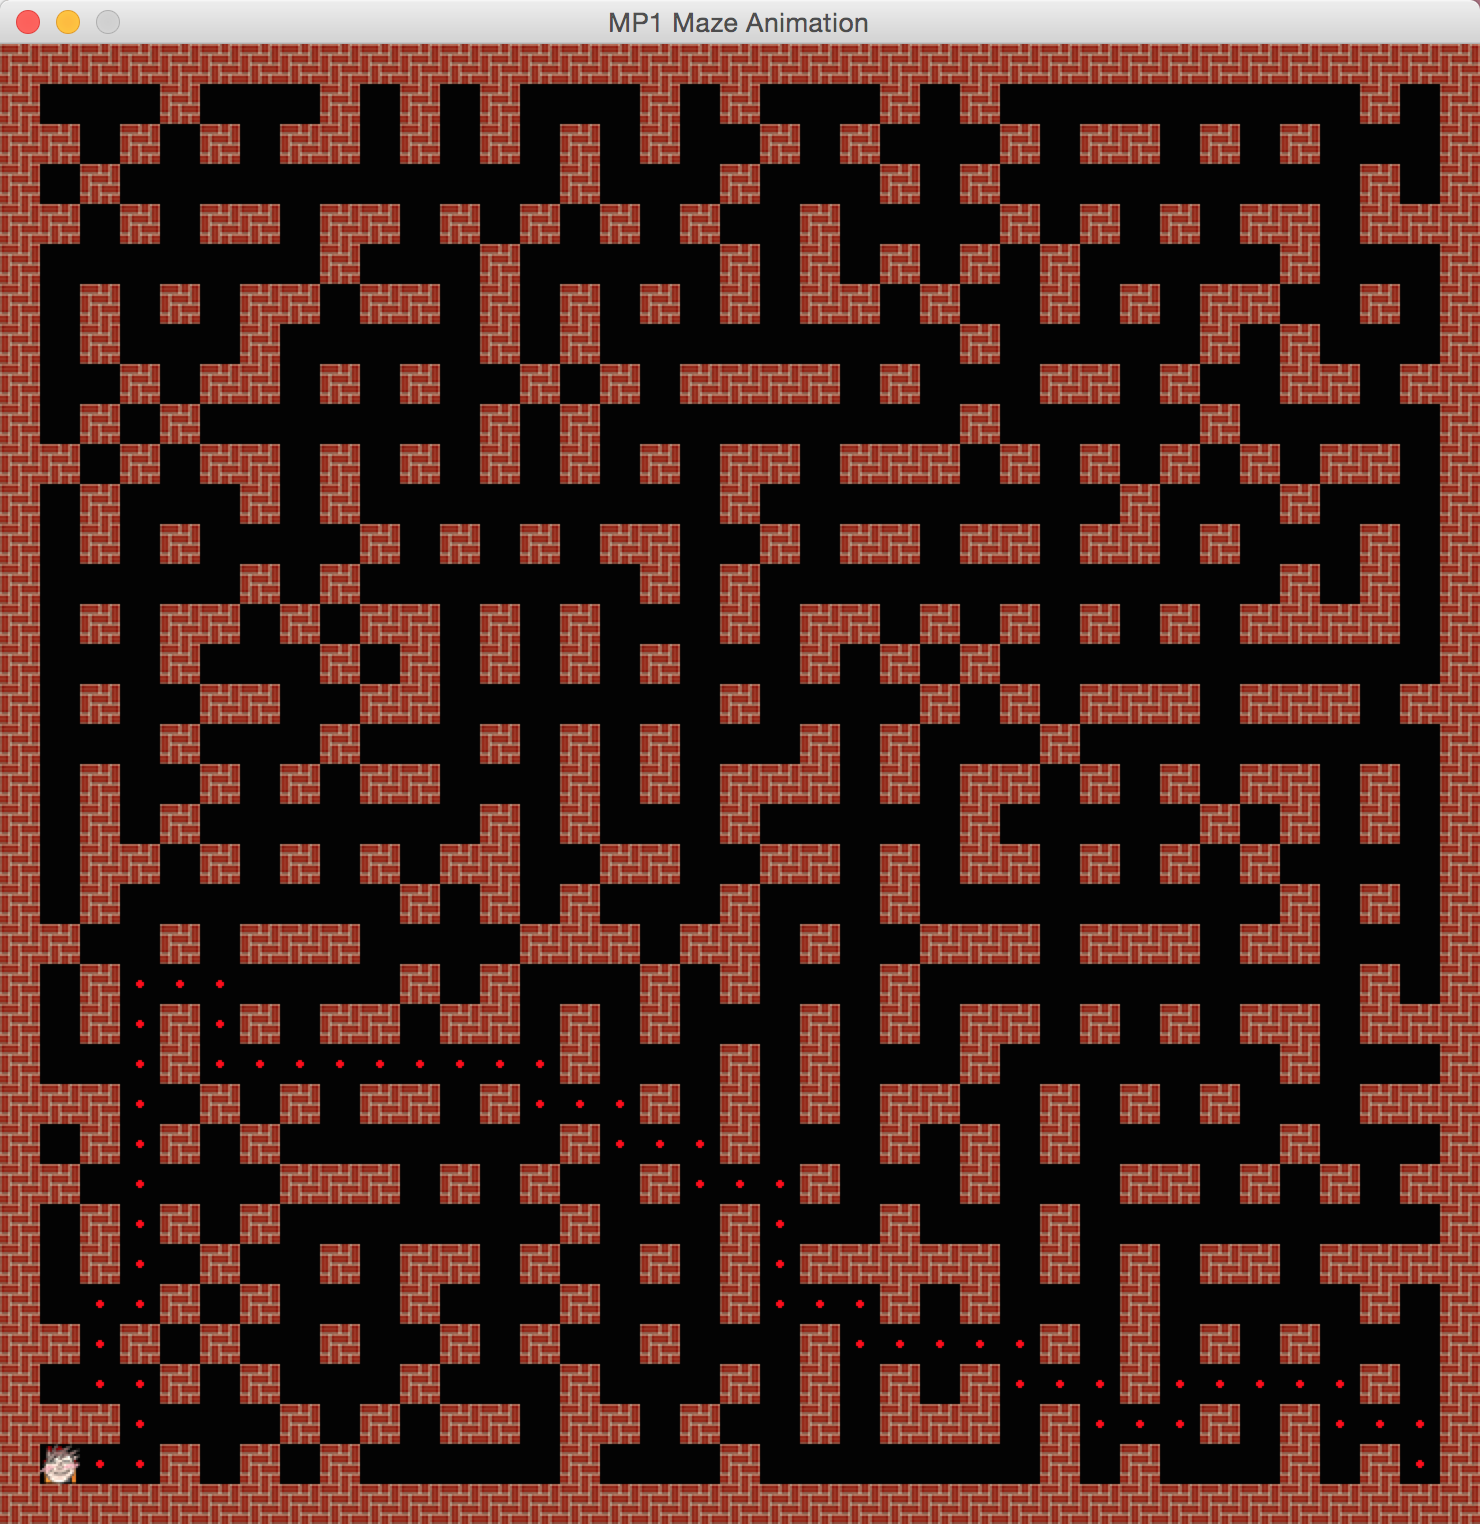
\includegraphics[width=0.3\textwidth]{graphics/bigMaze_alt21.png}

\paragraph{Results}
smallTurns.txt, move cost = 1, turn cost = 2, alternate heuristic\\
- Path cost: 74\\
- Number of nodes expanded: 144\\
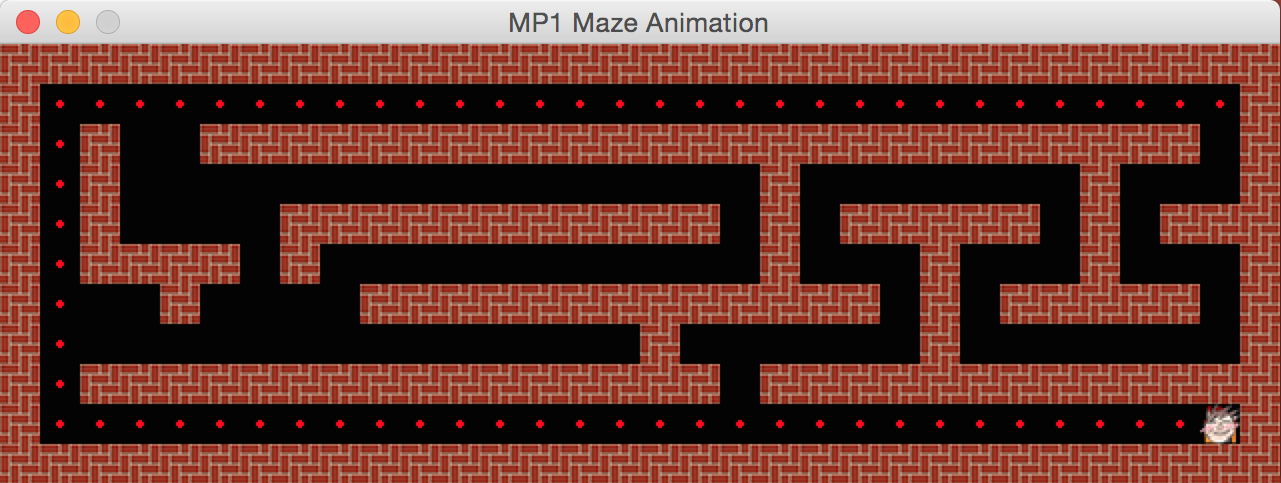
\includegraphics[width=0.3\textwidth]{graphics/smallTurn_alt12.png}

\paragraph{Results}
bigMaze.txt, move cost = 1, turn cost = 2, alternate heuristic\\
- Path cost: 118\\
- Number of nodes expanded: 533\\
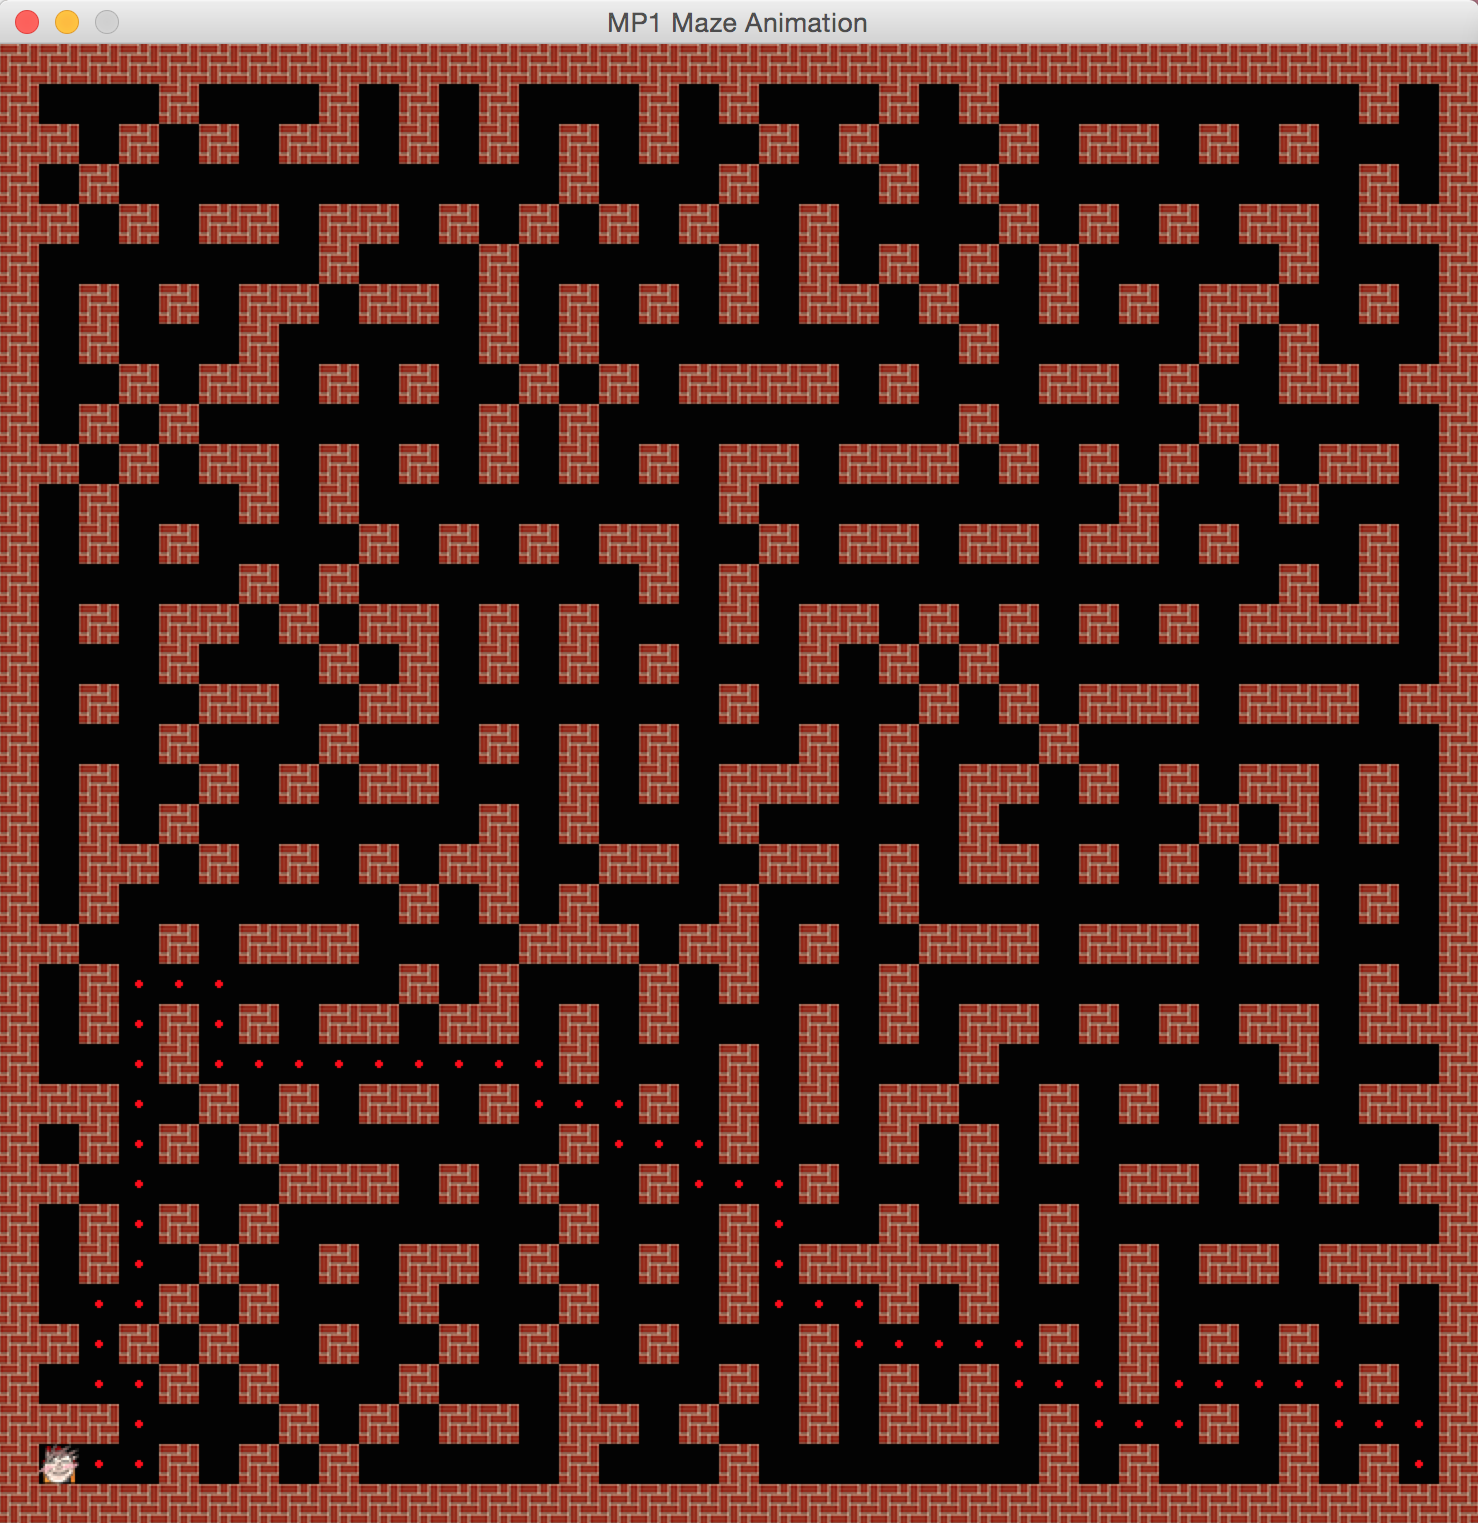
\includegraphics[width=0.3\textwidth]{graphics/bigMaze_alt12.png}

\subsection*{1.3}
\subsubsection*{A* search with ghosts}
In the case of ghosts, the environment is defined by the position of the ghosts and their current direction. In addition to walls, the algorithm has a constraint such that Pacman must avoid the position that ghosts will move to in the next turn. The algorithm also remembers the direction to relocate ghosts every turn, and to prevent Pacman from passing through ghosts. To illustrate, in two different cases such that ghosts are located at the same coordinate but have different directions, the future position of each ghost may be different, and therefore, the movement of Pacman is affected differently as well.

Therefore, this algorithm is modified based on the A* algorithm of 1.3 and stores in the heap tuples of the form (path cost from start to current coordinate + Manhattan distance from the current coordinate to goal, path cost from start to current coordinate, path from start to current coordinate, current coordinate, current coordinate of ghosts, current direction of ghosts, path records of ghost for animation: it is not necessary to store in the case without animation). Similar to our A* algorithm, the algorithm pops from the frontier the coordinate's tuple with the lowest "path cost + Manhattan distance". However, when examining Pacman's neighbors, the algorithm checks the ghost's position and direction, not only if neighbors have not been visited. In other words, if the state, in the form (coordinate of neighbor, positions of ghost in the next move, direction of ghosts), is not in the heap tuples of visited states, the algorithm adds the neighbor to the frontier. The algorithm then continues examining the frontier and expanding the coordinate with the lowest sum of current path cost and Manhattan distance heuristic, as described above.

To relocate a ghost every turn, the algorithm refers to its current position and direction. Let us say the direction is front. Firstly, the ghost searches its neighbor in the default direction, right. If the neighbor is not on the ghost's path (neither "g" nor "G"), it changes the direction to left. The process of examining whether neighbors are on the ghost's path and changing the direction will be repeated, in the order of right (default), left, rear, and front. If the neighbor is on the ghost's path, return the current direction at that time. In the case there is no path, the ghost takes the default direction after trying all the other directions, and does not update its position. In other words, neither the direction nor the position is changed. In the case that the ghost is at the end of a path, after examining the front, left, right, it will take the rear direction and move to the neighbor on its rear side. Using this method, it is possible to implement mazes with complicated ghost paths.

\paragraph{Results}
smallGhost.txt\\
- Path cost: 22\\
- Number of nodes expanded: 180\\
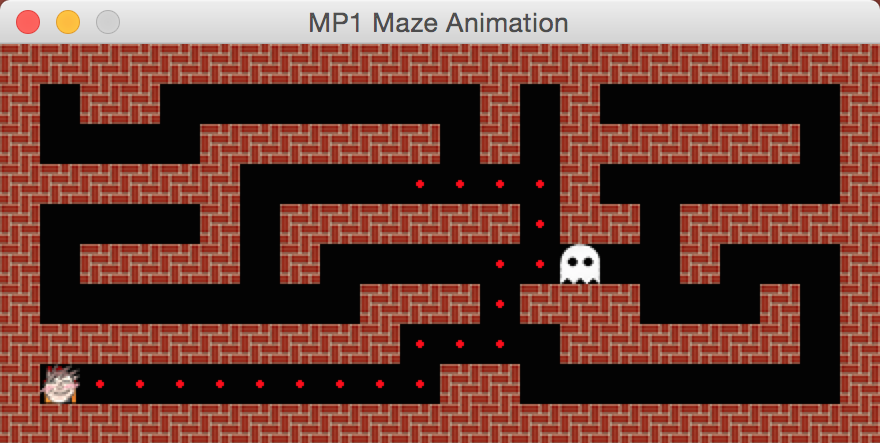
\includegraphics[width=0.3\textwidth]{graphics/smallGhosts.png}

\paragraph{Results}
mediumGhost.txt\\
- Path cost: 27\\
- Number of nodes expanded: 142\\
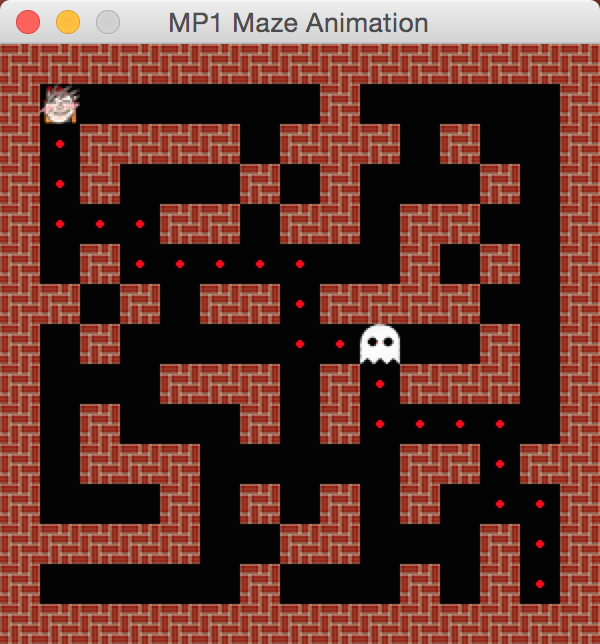
\includegraphics[width=0.3\textwidth]{graphics/mediumGhosts.png}
\columnbreak

\paragraph{Results}
bigGhost.txt\\
- Path cost: 71\\
- Number of nodes expanded: 590\\
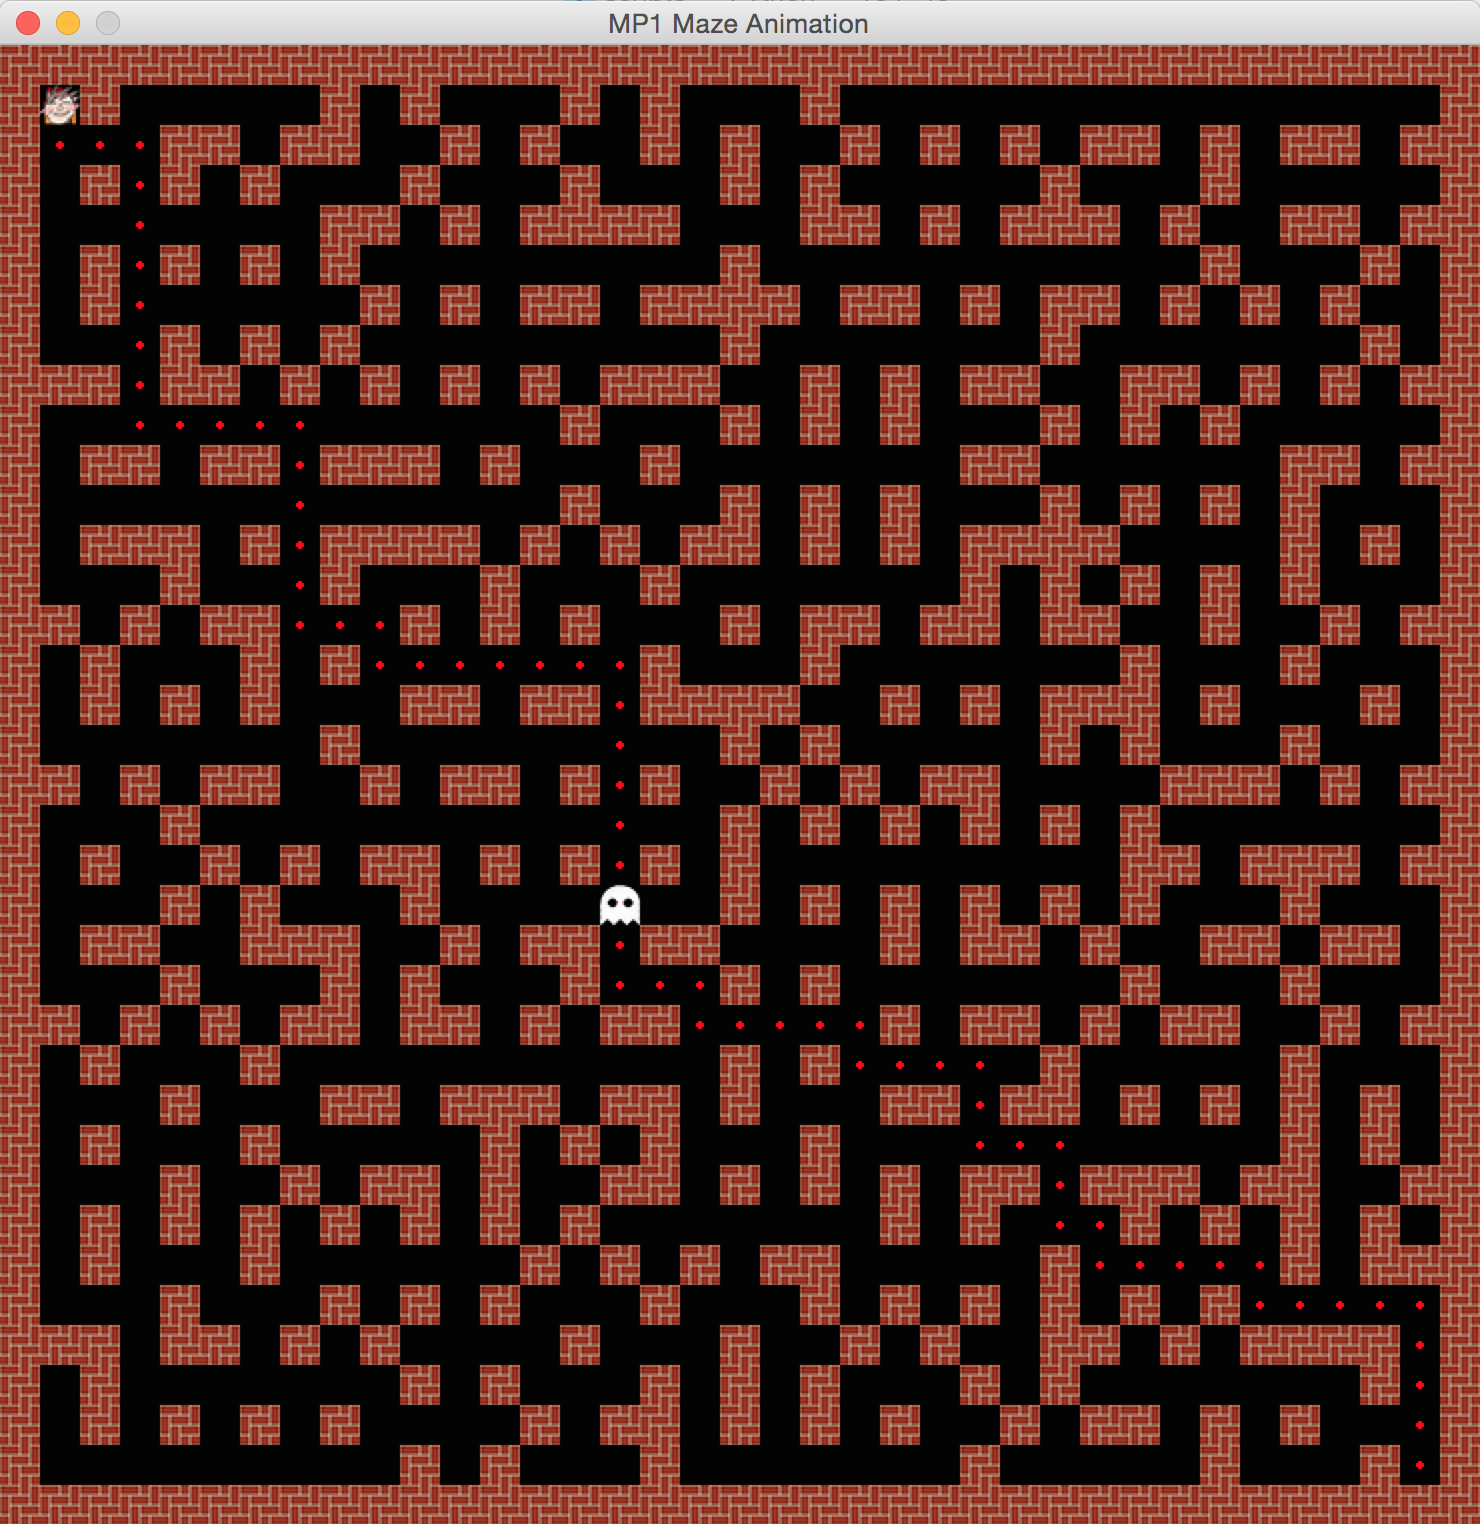
\includegraphics[width=0.5\textwidth]{graphics/bigGhosts.png}

\subsection*{Extra Credit}
First, by using the structure to store multiple ghosts' positions every turn, the algorithm can find a solution in the case with multiple ghosts. Also, using the method of relocating ghosts mentioned above in 1.3, we implemented the mazes such that each ghost has complicated paths: ghosts can curve frequently, never move, and even circulate. the initial direction of each ghost is chosen randomly. Once the initial directions are chosen, the algorithm can predict ghosts' movement, and therefore, can successfully find an optimized path. To demonstrate the code, we used the below map: multipleGhosts.txt. Finally, using the PyGame library, our program can display animation that shows Pacman finding a path to the goal(s). For parts 2.1 and 2.2, once Pacman visits each goal, they become gray. In the animation, we used images from these sources:\newline
Pacman: Private graphics of Mingyo Seo\newline
Goal: http://www.clipartbest.com/house-clip-art\newline
Wall: http://www.tutorialsforblender3d.com/Textures/ \newline Bricks-NormalMap/Bricks\_Normal\_1.html \newline
Ghost: https://www.iconfinder.com/icons/133161/ \newline enemy\_ghost\_icon \newline


\paragraph{Results}
multipleGhosts.txt\\
- Path cost: 77\\
- Number of nodes expanded: 840\\
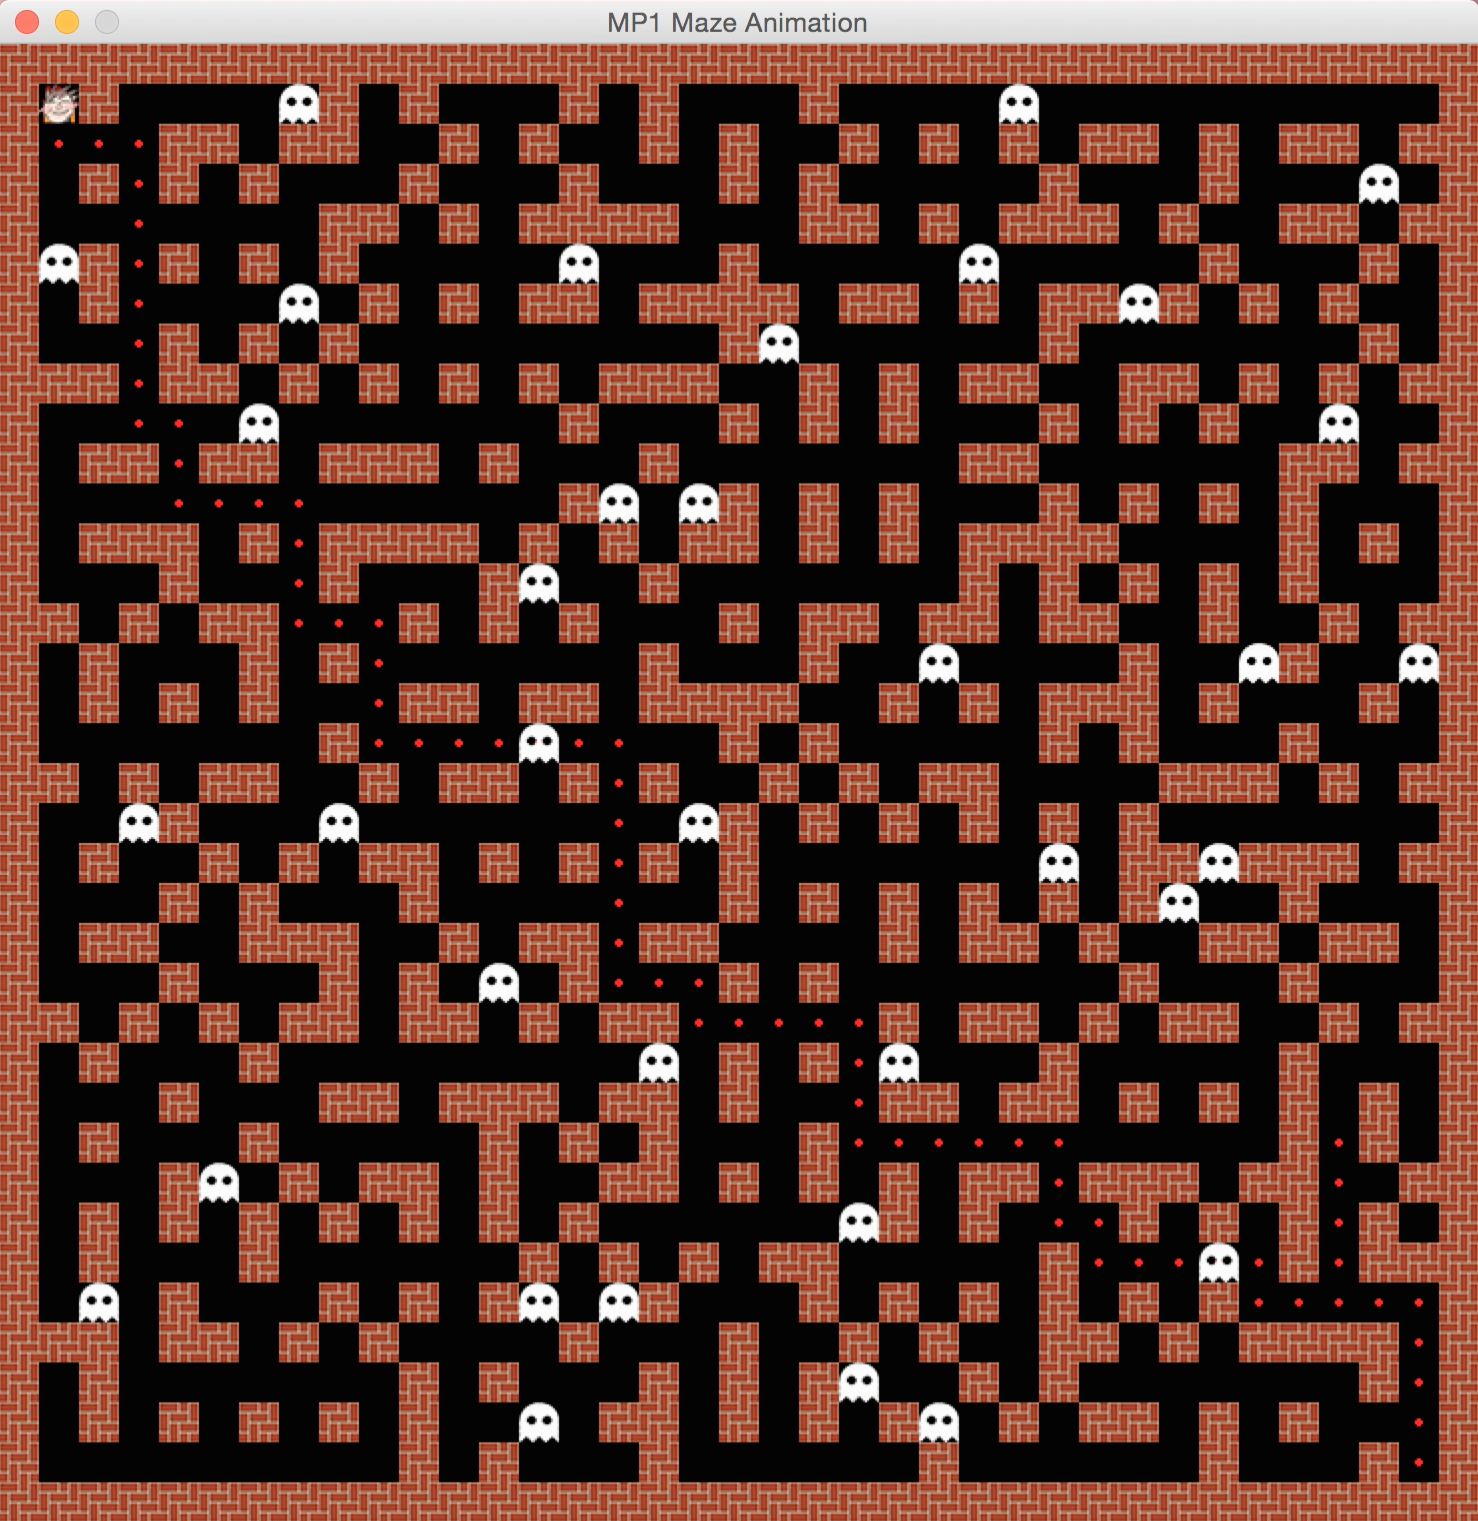
\includegraphics[width=0.5\textwidth]{graphics/multipleGhosts.png}
Demo Video Link: https://youtu.be/r9RzC-kf7EU

\end{multicols*}
